% !Mode:: "TeX:UTF-8"
% !TEX program  = xelatex
\documentclass[withoutpreface,bwprint]{cumcmthesis} 
\input{Misc/preamble.tex}
%以上为格式规定与包的引用,勿动。以下为正文内容,从标题开始

%标题
\title{Exploratory Deep Learning Models: Determining Optimal Cutting Parameters for a Microtome}

% “利用深度学习优化活检参数:通过迁移学习和实时反馈系统提高组织切片的准确性”
\renewcommand{\headrulewidth}{0pt} % 不显示页眉线
\renewcommand{\footrulewidth}{0pt} % 不显示页脚线\left( 
\begin{document}
 \maketitle
%英文摘要
\renewcommand{\abstractname}{Abstract}
\renewcommand{\keywords}{\textbf{Keywords:}}
\begin{abstract}
\begin{spacing}{1.15}

	This study investigates optimizing biopsy parameters through deep learning, utilizing the InceptionV3 model via transfer learning for assessing the quality of biomedical tissue sections. Experiments with various cutting angles identified optimal parameters that significantly improved tissue section quality. Additionally, image preprocessing studies showed that using original image data often resulted in better outcomes than using processed images.
    The research suggests further expanding classification methods, enhancing performance, investigating additional influencing factors, and dynamically adjusting slicing parameters. These proposals aim at developing fully automated histology instruments. The findings confirm the model's adaptability to various tissue types, highlighting its potential as a versatile tool in histopathology.

	% 本研究通过深度学习,利用迁移学习中的InceptionV3模型,探讨了如何优化活检参数,以评估生物医学组织切片的质量。通过对各种切割角度的实验,我们确定了可以显著提高组织切片质量的最佳参数。此外,图像预处理研究表明,使用原始图像数据通常比使用处理过的图像得到更好的结果。 研究建议进一步扩展分类方法,提高性能,研究更多影响因素,并动态调整切割参数。这些提议旨在开发全自动组织学仪器。研究结果证实了该模型对各种组织类型的适应性,突显了其在组织病理学中作为多功能工具的潜力。


% 	Keywords
% Deep Learning
% Biomedical Imaging
% Tissue Sectioning
% Histopathology
% Transfer Learning
% InceptionV3
% Image Preprocessing
% Cutting Angle Optimization
% Real-time Feedback Systems
% Automated Histology
%英文摘要内容
\end{spacing}
\large

\end{abstract}




%目录(前三行为目录格式调整)
%\cftsetindents{section}{0em}{2em}
%\cftsetindents{subsection}{2em}{3em}
%\cftsetindents{subsubsection}{4em}{4em}
\newpage
{
	\fontspec{Times New Roman}
	\tableofcontents
}
\newpage


%
%以下部分为正文内容
% \pagenumbering{arabic}
\section{Introduction and background}
\label{sec:introduction}


\subsection{Introduction}

\subsubsection{Project Overview}

This project addresses the critical task of optimizing the cutting parameters of a biological tissue slicer, an essential instrument in biomedical research and clinical diagnostics. The aim is to enhance the precision and efficiency of tissue sample preparation by identifying the optimal slicing conditions. Through the collection of tissue samples under various cutting parameters and subsequent artificial image classification, this study employs deep learning techniques to analyze and predict the most effective slicing parameters. This endeavor not only promises to improve the quality of tissue samples for microscopic examination but also to streamline the workflow in laboratories, thereby contributing to the advancement of biological and medical sciences.
% 这个项目解决了生物组织切片仪的关键任务,这是生物医学研究和临床诊断中的一个重要仪器。其目标是通过确定最佳切片条件来提高组织样本制备的精确性和效率。通过收集在不同切割参数下的组织样本,并进行人工图像分类,本研究采用深度学习技术来分析和预测最有效的切片参数。这个努力不仅有望改善显微镜检查的组织样本质量,还有望简化实验室的工作流程,从而促进生物和医学科学的进步。
\subsubsection{Objectives}

\begin{enumerate}
    \item Collect a comprehensive dataset of tissue samples sliced under different parameters.
    \item Employ artificial image classification to categorize the quality and characteristics of these samples.
    \item Develop and train a deep learning model capable of assessing tissue sample quality.
    \item Use the model's insights to determine the optimal cutting parameters for the tissue slicer.
    \item Validate the model's predictions through empirical testing and refinement.
\end{enumerate}

% \item 收集在不同参数下切割的组织样本的全面数据集。
% \item 使用人工图像分类来对这些样本的质量和特征进行分类。
% \item 开发和训练一个能够评估组织样本质量的深度学习模型。
% \item 利用模型的见解来确定组织切片仪的最佳切割参数。
% \item 通过实证测试和改进来验证模型的预测结果。
% \end{enumerate}

\subsubsection{Structure of the Report}

This project is organized into the following chapters, each designed to systematically explore the research background, methodologies, experimental work, results presentation, discussions and conclusions, as well as considerations for project management, sustainability, and health and safety:

\textbf{Introduction and Background} - This chapter outlines the project's objectives, goals, and structural arrangement. It provides a brief introduction to the motivation and necessity for the research, along with the technical protocols and specifications adopted.

\textbf{Literature Review} - An in-depth discussion on the use of biological tissue slicers, image classification, and deep learning in the preparation of biological samples. This section positions the current study within the context of existing research.

\textbf{Methodology and Theory} - Detailed descriptions of the experimental methods, theoretical frameworks, and the specific plans for data collection and processing are presented here.

\textbf{Experimental Work/Analytical Investigation/Design} - Describes the detailed steps of experimental design, implementation, and analytical investigation. It elaborates on the strategies and methods adopted to achieve the project's objectives.

\textbf{Presentation of Experimental or Analytical Results/Descriptions of Final Constructed Product} - This chapter showcases the experimental data, analysis results, or the final design product, providing detailed accounts of the experimental or design outcomes.

\textbf{Discussion and Conclusions} - The results are analyzed, and their scientific significance and practical value are discussed. This chapter also offers the research conclusions and suggests potential directions for future studies.

\textbf{Project Management, Consideration of Sustainability and Health and Safety} - Discusses strategies for project management, sustainability issues, and health and safety measures to ensure the research work is conducted efficiently and safely.

\textbf{References} - Lists all the bibliographic materials cited, supporting the research and providing the basis for the study.
% 本项目分为以下几个章节,每个章节都旨在系统地探索研究背景、方法论、实验工作、结果展示、讨论和结论,以及项目管理、可持续性和健康安全方面的考虑:

% \textbf{引言和背景} - 本章概述了项目的目标、目标和结构安排。它简要介绍了研究的动机和必要性,以及采用的技术协议和规范。

% \textbf{文献综述} - 对生物组织切片、图像分类和深度学习在生物样本制备中的应用进行深入讨论。本节将当前研究定位于现有研究的背景下。

% \textbf{方法和理论} - 详细描述了实验方法、理论框架以及数据收集和处理的具体计划。

% \textbf{实验工作/分析调查/设计} - 描述了实验设计、实施和分析调查的详细步骤。详细阐述了实现项目目标所采用的策略和方法。

% \textbf{实验或分析结果展示/最终构建产品描述} - 本章展示了实验数据、分析结果或最终设计产品,详细描述了实验或设计结果。

% \textbf{讨论和结论} - 对结果进行分析,讨论其科学意义和实际价值。本章还提供研究结论,并提出未来研究的潜在方向。

% \textbf{项目管理、可持续性和健康安全考虑} - 讨论项目管理策略、可持续性问题和健康安全措施,以确保研究工作的高效和安全进行。

% \textbf{参考文献} - 列出所有引用的文献资料,支持研究并为研究提供基础。

\subsubsection{Assumptions and Technical Specifications}

The project is based on several key assumptions and technical protocols, which are:

\begin{enumerate}
    \item The consistency in tissue sample properties across different batches.
    \item The reliability and precision of the biological tissue slicer and imaging equipment.
    \item The adequacy of the deep learning model in interpreting complex biological image data.
\end{enumerate}
Technical specifications regarding the tissue slicer settings, image classification criteria, and deep learning architecture are detailed in \textbf{Methodology and Theory}.
% 该项目基于几个关键假设和技术协议,包括:

% \begin{enumerate}
%     \item 不同批次之间组织样本性质的一致性。
%     \item 生物组织切片仪和成像设备的可靠性和精确性。
%     \item 深度学习模型在解释复杂生物图像数据方面的充分性。
% \end{enumerate}
% 有关组织切片仪设置、图像分类标准和深度学习架构的技术规格详见方法和理论。

\subsection{Background}

\subsubsection{Importance of Tissue Sample Quality}

High-quality tissue samples are pivotal for accurate diagnosis and research. The quality of a tissue sample can significantly affect the results of histological analysis, making the optimization of slicing parameters a crucial endeavor.

\subsubsection{Advancements in Image Classification and Deep Learning}

Recent advancements in image classification and deep learning have opened new avenues for automating and enhancing the analysis of biological samples. By leveraging these technologies, it is possible to achieve greater accuracy and efficiency in identifying optimal tissue slicing parameters.

\subsubsection{Gap in Current Research}

While there have been significant strides in both biological sample preparation and computational analysis, a gap remains in integrating these approaches to optimize tissue slicing parameters. This project aims to bridge this gap by developing a predictive model that can guide the adjustment of slicing conditions for optimal outcomes.

% \subsection{背景}

% \subsubsection{组织样本质量的重要性}

% 高质量的组织样本对于准确的诊断和研究至关重要。组织样本的质量可以显著影响组织学分析的结果,因此优化切片参数是一项关键的工作。

% \subsubsection{图像分类和深度学习的进展}

% 图像分类和深度学习的最新进展为自动化和增强生物样本分析开辟了新的途径。通过利用这些技术,可以在识别最佳组织切片参数方面实现更高的准确性和效率。

% \subsubsection{当前研究中的差距}

% 尽管在生物样本制备和计算分析方面取得了重大进展,但在整合这些方法以优化组织切片参数方面仍存在差距。本项目旨在通过开发一个预测模型来填补这一差距,该模型可以指导调整切片条件以获得最佳结果。

\section{Literature review}

This literature review examines the convergence of technologies in biological tissue slicing, with a particular focus on the application of image classification and deep learning to optimize slicing parameters. It aims to highlight significant advancements, identify gaps in current methodologies, and set the groundwork for the proposed project.

% 这篇文献综述探讨了生物组织切片中技术的融合,特别关注图像分类和深度学习在优化切片参数方面的应用。它旨在突出重要的进展,确定当前方法学中存在的差距,并为拟议的项目奠定基础。
\subsection{切片机与显微镜的选择}
%组织切片和图像获取的技术背景   这里写切片机和显微镜的技术参数和采集手册及方法


近年来,随着科技的发展,自动切片机的出现能够显著简化切片操作和提高切片质量。

M在《Improved reproducibility in preparing precision-cut liver tissue slices》一文中提出,使用新型徕卡振动刀片切片机可以提高大鼠、小鼠和人体组织切片的准确性和重现性。-----------



在本次实验中,使用epredia提供的HM355S机器进行切片处理。该机器是一款热门的用于生物组织切片研究的设备,有不少实验和论文都使用了这款设备进行切片处理。

Elzbieta Klimuszko 使用过HM355S机器,以牙齿作为标本进行切片操作,探究牙釉质中的钙镁含量。-------------
https://link.springer.com/article/10.1007/s10266-018-0353-6


Andelko Hrzenjak使用HM355S机器,对病变的子宫内膜组织进行切片操作,研究子宫内膜癌的发生机制。-------------
https://www.sciencedirect.com/science/article/pii/S1525157810605685

同样,对于显微镜的选择也是至关重要的。在本次实验中,使用了来自Keyence公司的VHX7000显微镜进行图像采集。他不仅能采集生物组织切片的图像(小鼠前列腺细胞
https://www.frontiersin.org/journals/oncology/articles/10.3389/fonc.2022.943846/full
),


还能采集无机物(如陶瓷,玻璃)的表面图像。
https://www.sciencedirect.com/science/article/abs/pii/S010956412300204X
https://www.taylorfrancis.com/chapters/edit/10.1201/9781003023555-130/looking-foundations-structural-glass-digital-microscope-veer

实验中将使用HM355s切片机和VHX7000显微镜进行切片和图像采集。

% 希望通过自动化操作过程可可靠地控制切片的质量,增加高质量标本的产量,减少次品标本的数量。然而,不同组织样本的最佳切割参数各不相同。确定特定组织的最佳切割参数仍然是一个挑战。

% \subsection{Image Classification for Tissue Analysis}

% %用于组织分析的图像分类   这里写图像分类的技术背景和方法


\subsection{关于切片组织的深度学习}

%深度学习在生物医学应用中的应用   这里写深度学习的技术背景和方法

深度学习技术在生物医学领域的应用已经取得了显著进展。深度学习模型在图像分类、目标检测和分割等任务中表现出色,为生物医学实验室的研究和诊断提供了强大的工具。

Lorena Guachi-Guachi 提出了一种使用cnn网络对组织切片进行识别并进行修整。

应用于切片术的卷积神经网络:识别石蜡包埋组织块的修剪末端切割程序
https://www.sciencedirect.com/science/article/abs/pii/S0952197623011478


在Biomedical Texture Analysis一书中,Vincent Andrearczyk提出了一种专门用于纹理分析的cnn架构,相比其它传统架构能够显著提高生物组织的分类准确性。

第 4 章-纹理分析中的深度学习及其在组织图像分类中的应用
https://www.sciencedirect.com/science/article/abs/pii/B9780128121337000041


Yan Xu提出,从大型自然图像数据库 ImageNet 训练的 CNN 中提取的特征能够转移到组织病理学图像中,这为我们实现迁移学习提供了一种可行的思路。

通过深度卷积激活特征进行大规模组织病理学图像分类、分割和可视化
https://link.springer.com/article/10.1186/s12859-017-1685-x

根据以上文献,深度学习技术在组织切片的图像分类和分析中具有广泛的应用前景。通过利用深度学习模型,可以实现对组织样本的高效识别和分类,为优化切片参数提供有力支持。


% \subsection{Integration of Deep Learning for Optimizing Tissue Slicing Parameters}

% %整合深度学习以优化组织切片参数   这里写深度学习在优化切片参数中的应用


\FloatBarrier % Now figures cannot float above section title


%% 草稿
% 历史上,组织切片主要依赖于手工技术,这既耗时又容易产生变异。近年来,自动切片机的发展旨在解决这些问题。然而,通过整合先进的图像分析和机器学习技术来优化切片参数仍然是一个挑战,很少有人涉及到这个领域。

% 生物医学成像领域在图像分类方面取得了显著的进展,特别是引入机器学习和深度学习模型。这些技术在高精度识别和分类组织特征方面显示出潜力,为自动评估组织切片质量提供了可能的途径。

% 深度学习因其处理和分析复杂数据集的能力而越来越受到认可,从而提高了生物医学实验室的效率。值得注意的是,一些研究已经开始探索深度学习在优化生物医学设备参数方面的潜力,尽管在组织切片优化方面的研究仍然有限。

% 尽管组织切片、图像分类和深度学习各自取得了显著进展,但在整合它们以优化组织切片参数的研究仍然很少。这为本项目提供了一个独特的机会,通过开发一个综合模型,将这些技术协同应用,为该领域做出贡献。

% 尽管深度学习和图像分类在生物医学应用中具有潜在的能力,但它们在优化组织切片参数方面的应用仍未得到充分探索。本项目旨在填补这一空白,通过开发一个基于深度学习的模型,预测最佳切片条件,从而提高组织样本在研究和诊断中的质量。


% 文献综述强调了通过整合深度学习和图像分类技术改进组织切片的重要潜力。通过解决已确定的研究差距,本项目有望对组织样本制备的效率和准确性做出有意义的贡献,对生物医学研究和诊断具有广泛的影响。

% \section{Literature review}


这篇文献综述探讨了生物组织切片中技术的融合,特别关注图像分类和深度学习在优化切片参数方面的应用。它旨在突出重要的进展,确定当前方法学中存在的差距,并为拟议的项目奠定基础。

\subsection{切片机与显微镜}

近年来,自动切片机的出现显著简化了切片过程,并提高了切片的质量。

Zimmermann在文章"Improved reproducibility in preparing precision-cut liver tissue slices"中,主张使用新的Leica振动刀来提高大鼠、小鼠和人体组织切片的精度和重复性 \cite{LR.1}。

在这个实验中,我们使用Epredia提供的HM355S切片机进行切片。这台机器是生物组织切片研究的流行设备,许多实验和论文都使用了这台设备进行切片。

Elzbieta Klimuszko使用HM355S切片机切割牙齿,以研究牙釉质中的钙和镁含量 \cite{LR.2}。

Andelko Hrzenjak也使用HM355S切片机切割病理性子宫内膜组织,以研究子宫内膜癌发展的机制 \cite{LR.3}。

同样,显微镜的选择也至关重要。在这个实验中,我们使用Keyence的VHX7000显微镜进行图像采集。它能够捕获生物组织切片的图像(例如,小鼠前列腺细胞 \cite{LR.4}),以及无机材料(如陶瓷 \cite{LR.5},玻璃 \cite{LR.6})。

实验将使用HM355s切片机和VHX7000显微镜进行切片和图像采集。这种设置确保了设备选择和技术应用的最佳配合,以提高组织切片过程的精度和效率,支持研究项目的总体目标。

% \subsection{深度学习的原理}







\subsection{医学图像分类-基于卷积神经网络}

对于医学图像分类问题来说,以卷积神经网络为主的深度学习模型已经被证实是最有效的方法之一。\cite{5.1 1}

卷积神经网络(CNN)是一种深度学习模型,尤其擅长处理图像数据。它通过一系列卷积层自动学习空间层次的特征,无需手动特征提取。一个典型的CNN模型包括卷积层、池化层、全连接层等\cite{DL.4}。一个典型的CNN架构如下所示:\cite{4.30 1}


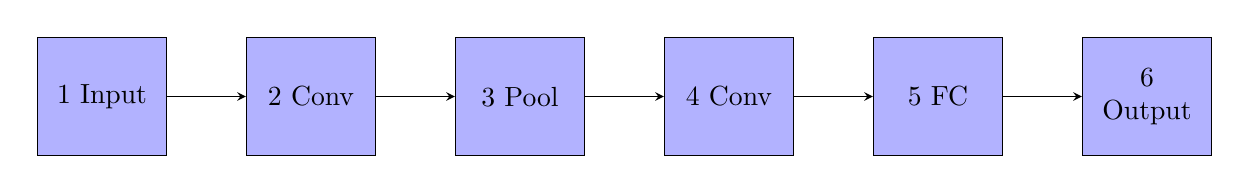
\begin{tikzpicture}[
    node distance=1cm and 0.5cm,
    block/.style={rectangle, draw, text width=4em, text centered, minimum height=15mm, fill=blue!30},
    arrow/.style={->,>=stealth}
]

% Define nodes in a matrix
\matrix [column sep=10mm, row sep=10mm] {
  \node (n1) [block] {1 Input}; & \node (n2) [block] {2 Conv}; & \node (n3) [block] {3 Pool} ;& \node
  (n4) [block] {4 Conv};    & \node (n5) [block] {5 FC};   & \node (n6) [block] {6 Output}; \\
};

% Connect nodes
\draw [arrow] (n1) -- (n2);
\draw [arrow] (n2) -- (n3);
\draw [arrow] (n3) -- (n4);
\draw [arrow] (n4) -- (n5);
\draw [arrow] (n5) -- (n6);
\end{tikzpicture}

在这个模型中:

\textbf{卷积层(Conv)}:这是CNN的核心层,负责从图像中提取特征。

\textbf{池化层(Pool)}:这些层用于减少特征图的维度,从而降低计算负载。

\textbf{全连接层(FC)}:这些层整合了卷积层和池化层提取的特征,用于分类或回归分析,最终导致输出。

对于一个典型的训练CNN的方法,包括前向传播、损失计算、反向传播和权重更新的过程。\cite{4.30 2}
\begin{enumerate}
    \item 前向传播:输入数据通过网络的每一层,直到输出层。
    \item 计算损失:使用损失函数(如交叉熵损失)计算网络输出和实际标签之间的差异。
    \item 反向传播:计算损失函数关于网络权重的梯度。
    \item 权重更新:使用梯度下降算法或其变种(如Adam或RMSprop)来更新网络权重,目标是减少损失函数的值。
\end{enumerate}
一旦训练完成,CNN可以用来预测新的、未见过的图像的标签。CNN的独特之处在于它们能够自动且高效地学习不同层次的抽象特征,使它们对于涉及复杂图像数据的任务非常有效,如医学图像分析,其中准确性和细节至关重要。\cite{4.30 3}

\subsection{医学图像分类-基于迁移学习}

对于CNN模型来说,一个显而易见的提升深度学习性能的方法是迁移学习。Sudhakar指出,在面对复杂分类问题比如恶意软件分类问题时,拥有大量参数的深度学习模型性能会显著优于传统机器学习模型。然而,由于深度学习模型需要大量的数据和计算资源,迁移学习成为了一个重要的解决方案。\cite{5.1 2}

迁移学习是一种机器学习方法,通过将一个模型训练的知识迁移到另一个模型上,从而加速训练过程。迁移学习的核心思想是利用源领域的知识来帮助目标领域的学习。\cite{4.30 4}

对于CNN模型,有几种迁移学习的方法,如微调和特征提取:

\textbf{微调}涉及调整预训练模型的参数以适应新任务。这通常包括在新数据上重新训练一些卷积层和全连接层,使模型能够将特征微调到新数据集的特定特性。\cite{4.30 5}

\textbf{特征提取}涉及使用预训练模型作为固定的特征提取器,其中只有全连接层在新数据上进行训练。在这种方法中,卷积层保持其学习的权重,并仅用于提取特征,这些特征然后被新训练的分类器层用于执行特定于新数据集的任务。\cite{4.30 6}

在Kora的研究中\cite{5.1 3},迁移学习能够消除从头开始训练模型的需要,并且能够在保证医学切片识别准确率的情况下,需要更少的数据。这种方法在医学图像分类问题中具有广泛的应用前景。

\subsection{关于切片组织的深度学习}

在生物医学领域,深度学习技术的应用已取得了显著的进步。深度学习模型在图像分类、对象检测和分割等任务中表现出色,为生物医学实验室的研究和诊断提供了强大的工具。

Lorena Guachi-Guachi 提出了一种利用 CNN 网络识别和精炼组织切片的方法。这种方法代表了深度学习的创新应用,可以提高组织准备和分析的精度 \cite{LR.7}。

在《生物医学纹理分析》一书中,Vincent Andrearczyk 介绍了一种专为纹理分析设计的 CNN 架构,与传统架构相比,这种架构显著提高了生物组织分类的准确性 \cite{LR.8}。这一发展展示了深度学习提高组织特性详细分析的潜力,这对于准确的诊断和研究至关重要。

Yan Xu 提出,从在大型自然图像数据库 ImageNet 上训练的 CNN 中提取的特征可以转移到组织的病理学图像上 \cite{LR.9}。这为实施转移学习提供了一种可行的方法,可以大大提高组织图像分类和分析的效率。

根据文献,深度学习技术在组织切片的图像分类和分析中有广阔的应用前景。通过利用深度学习模型,可以实现组织样本的有效识别和分类,为优化切片参数提供了强大的支持。

这一部分强调了深度学习对组织切片领域的变革性影响,预示着在组织学分析的准确性和实用性方面的显著改进。

\FloatBarrier % Now figures cannot float above section title

% \section{Methodology and theory}
\label{sec:problem_description}
\subsection{Subsection 2.1}
\subsection{Subsection 2.2}



\section{Experimental work/analytical investigation/ design}
\FloatBarrier
 
% \section{Experimental work/ analytical investigation/ design}


\subsection{采集数据}
在本实验中,我们使用了预先从生物实验室制备并染色的石蜡包埋组织切片(\autoref{label:sample})。使用HM355s自动切片机,按照操作手册,以不同切削角度进行切片,记录切削参数。切片后,组织样本放置于平面上并干燥(\autoref{fig:采集样本}),随后在VHX7000显微镜下进行成像,以捕获电子图像数据(\autoref{fig:显微镜})。

如\autoref{fig:machine}所示的切片机(以牙齿为例),如\autoref{fig:cutting_machine} \cite{4.1}所示,是为精确切割而设计的。在这个设置中,原始样本被安全地固定用于切割,由精确的刀片执行切割。切割后,切片在指定的表面上由水流展开和平坦,然后移动到存储区域。从存储区域取出并干燥后,切片被放置在显微镜舞台上,显微镜自动对焦并捕获图像数据。切割参数如下:模式设置为连续,进给速度为5.0,修整值为25,速度设定为32,水流速度为7.5,水温约为36摄氏度。切割角度在8到12度之间。显微镜的放大倍数是20x20,分辨率是2880x2160。

%在这不要提三个点的鱼的肺泡组织,在后面作为模型二次验证和增强使用。


\begin{figure}[H]
    \centering
    \begin{minipage}{0.35\textwidth}
        \centering
        \includegraphics[width=\textwidth]{./fig/machine - 副本.jpg}
        \caption{切片机}
        \label{fig:machine}
    \end{minipage}
    \begin{minipage}{0.35\textwidth}
        \centering
        \includegraphics[width=\textwidth]{./fig/10266_2018_353_Fig1_HTML.jpg}
        \caption{切割过程}
        \label{fig:cutting_machine}
    \end{minipage}
\end{figure}
% https://link.springer.com/article/10.1007/s10266-018-0353-6


% 在切削过程中,从切角为8度开始(如\autoref{fig:machine}中的angle of inclination),每次增加0.5度,直到切角为12度。切片机在切片过程中保持给进速度为25,厚度为1。

\begin{figure}[H]
    \centering
    \begin{minipage}{0.3\textwidth}
        \centering
        \includegraphics[width=\textwidth]{./fig/sample - 副本.jpg}
        \caption{原始样本}
        \label{label:sample}
    \end{minipage}
    \begin{minipage}{0.3\textwidth}
        \centering
        \includegraphics[width=\textwidth]{./fig/采集样本.jpg}
        \caption{切片}
        \label{fig:采集样本}
    \end{minipage}
    \begin{minipage}{0.35\textwidth}
        \centering
        \includegraphics[width=\textwidth]{./fig/显微镜 - 副本.jpg}
        \caption{显微镜}
        \label{fig:显微镜}
    \end{minipage}
\end{figure}

%图片需要后续更改为卵巢的


% 样本示例如\autoref{fig:sample9.5}所示。

% \begin{figure}
%     \centering
%     \includegraphics[width=0.8\textwidth]{./fig/sample9.5.jpg}
%     \caption{切角9.5度的样本}
%     \label{fig:sample9.5}
% \end{figure}


\subsection{标注数据}

对于这个实验,数据集是根据组织切片的质量进行标记的。总的来说,生物组织的质量被分为两个主要类别:正常和不良。对收集的数据进行进一步分析,发现了常见的缺陷 - 切片上存在垂直或水平的白色皱纹,这明显表明切片无法使用。鉴于这些缺陷的独特性质,它们被分类为两个额外的特定类别:\textbf{水平线}(见\autoref{fig:horizental_line})和\textbf{垂直线}(见\autoref{fig:vertical_line})。

\begin{figure}[H]
    \centering
    \begin{minipage}{0.33\textwidth}
        \centering
        \includegraphics[width=\textwidth]{./fig/sample_1/horizental_line - 副本.jpg}
        \caption{horizental line}
        \label{fig:horizental_line}
    \end{minipage}
    \begin{minipage}{0.33\textwidth}
        \centering
        \includegraphics[width=\textwidth]{./fig/sample_1/vertical_line - 副本.jpg}
        \caption{vertical line}
        \label{fig:vertical_line}
    \end{minipage}
\end{figure}

此外,考虑到有一部分图片在采样时存在明显的旋转角度,这种情况下,我们也将其单独分为一类,称为slope(如图\autoref{fig:slope})。最后,对于剩下的图片,我们将其标注为other(如图\autoref{fig:other})。

\begin{figure}[H]
    \centering
    \begin{minipage}{0.32\textwidth}
        \centering
        \includegraphics[width=\textwidth]{./fig/sample_1/slope.jpg}
        \caption{slope}
        \label{fig:slope}
    \end{minipage}
    \begin{minipage}{0.32\textwidth}
        \centering
        \includegraphics[width=\textwidth]{./fig/sample_1/other.jpg}
        \caption{other}
        \label{fig:other}
    \end{minipage}
    \begin{minipage}{0.32\textwidth}
        \centering
        \includegraphics[width=\textwidth]{./fig/sample_1/normal.jpg}
        \caption{normal}
        \label{fig:normal}
    \end{minipage}
\end{figure}

正常的符合观察要求的切片如\autoref{fig:normal}所示。

对于每一张图片,我们需要将其标注为以上五个类别中的一个。这将作为我们的数据集,用于训练模型。

\subsection{模型1:简单CNN网络与原始图像}

对于一个新的数据集,其中模型的适当复杂度与给定图像复杂度的不确定性,首先采用基本的CNN架构来评估数据集的特性和图像的复杂性。
\begin{table}[H]
\centering
\caption{Configuration of the simple CNN model}
\begin{tabular}{ccccc}
    \toprule
    \textbf{Layer Type} & \textbf{Configuration 1a} & \textbf{Configuration 1b} & \textbf{Configuration 1c} \\
    \midrule
    Input Layer & - & - & - \\
    Conv Layer 1 & Conv3-32 (relu) & Conv3-16 (relu) & Conv3-32 (relu) \\
    Pooling Layer 1 & MaxPooling & MaxPooling& MaxPooling \\
    Conv Layer 2 & Conv3-32 (relu) & Conv3-32 (relu) & Conv3-32 (relu) \\
    Pooling Layer 2 & MaxPooling & MaxPooling& MaxPooling \\
    Conv Layer 3 & Conv3-32 (relu) & Conv3-64 (relu) & Conv3-32 (relu) \\
    Pooling Layer 3 & MaxPooling & MaxPooling& MaxPooling \\
    Flattening Layer & Flatten() & Flatten() & Flatten() \\
    FC(Full connect) & Dense(128, relu) & Dense(128, relu) & Dense(256, relu) \\
    Output Layer & - & - & - \\
    \bottomrule
\end{tabular}
\label{tab:cnn_simple_configuration}
\end{table}

简单CNN模型的配置在\autoref{tab:cnn_simple_configuration}中概述。这些初始模型,标记为配置1a、1b和1c,根据卷积层中的神经元数量和全连接层中的神经元大小进行变化。配置1a和1b根据卷积层中的神经元数量有所不同,而配置1c则在全连接层中的神经元大小上与配置1a有所不同。

预处理步骤包括将数据集分为训练集(80%)和测试集(20%)。在输入层,图像尺寸减半(从2880x2160到1440x1080),并对数据进行归一化。

在训练过程中,使用Adam优化器和交叉熵损失函数,实现早停以避免过拟合。

下面的图表显示了模型1a、1b和1c在训练周期中的准确性和损失。

\begin{figure}[H]
    \centering
    \begin{minipage}{0.49\textwidth}
        \centering
        \includegraphics[width=\textwidth]{./fig/model1/accuracy11.eps}
        \caption{Model 1 accuracy}
        \label{fig:model11_acc}
    \end{minipage}
    \begin{minipage}{0.49\textwidth}
        \centering
        \includegraphics[width=\textwidth]{./fig/model1/loss11.eps}
        \caption{Model 1 loss}
        \label{fig:model11_loss}
    \end{minipage}
\end{figure}


从图表中可以看出,模型1a、1b和1c的训练准确性逐渐增加,随着时间的推移趋于稳定,而训练损失则逐渐减少,接近零。这表明模型从训练数据中学习得相对良好。然而,对于验证集,所有三个模型的准确性在80%到85%的范围内稳定,而在某些情况下,验证损失相对较高,特别是在模型1a中,它接近2.5并显示出显著的波动。这表明存在一定程度的过拟合,即模型在训练数据上的表现优于在未见过的数据上。值得注意的是,模型1c在验证损失方面表现最好,表明其结构或参数调整可能更有效地提高泛化能力。

这里过拟合的可能原因是模型的复杂度相对于数据集的复杂度不足,表明模型可能没有有效地从数据中提取特征。尽管模型在训练集上达到了高准确性和低损失,但它们在验证集上的泛化能力需要增强。

为了提高模型的准确性,考虑对图像进行预处理并手动帮助模型进行特征提取可能是有益的,这有助于模型更好地泛化到新数据。

\subsection{图像预处理改进}

在模型性能不佳的情况下,可能是由于图像的复杂性阻碍了模型有效提取重要特征。因此,考虑使用边缘检测和阈值分割等图像预处理技术,以突出模型识别的所需特征,并减少无关特征和噪声,从而提高后续深度学习模型的准确性。

\subsubsection{边缘检测}

如3.2.1节所述,边缘检测的原理涉及识别像素强度(梯度)的变化,以确定图像内的边缘。

在进行边缘检测之前,首先应用一个初始预处理步骤——高斯模糊。高斯模糊的理由是它有助于减少图像中的噪声,平滑梯度过渡,并降低检测到假边缘的可能性,从而提高边缘检测的准确性\cite{4.3}。我们试验了21、41、61和81大小的高斯核,分别对应于图像宽度的1%、2%、3%和4%。

下面显示了高斯模糊后的图像。为了更好地演示高斯核大小对边缘检测的影响,模糊后使用Sobel算子计算边缘并增加50个单位的亮度以提高可见性。

\begin{figure}
    \centering
    \begin{minipage}{0.24\textwidth}
        \centering
        \includegraphics[width=\textwidth]{./fig/gausssian/blurred21.jpg}
        \caption*{k=21}
        \label{fig:blurred21}
    \end{minipage}
    \begin{minipage}{0.24\textwidth}
        \centering
        \includegraphics[width=\textwidth]{./fig/gausssian/blurred41.jpg}
        \caption*{k=41}
        \label{fig:blurred41}
    \end{minipage}
    \begin{minipage}{0.24\textwidth}
        \centering
        \includegraphics[width=\textwidth]{./fig/gausssian/blurred61.jpg}
        \caption*{k=61}
        \label{fig:blurred61}
    \end{minipage}
    \begin{minipage}{0.24\textwidth}
        \centering
        \includegraphics[width=\textwidth]{./fig/gausssian/blurred81.jpg}
        \caption*{k=81}
        \label{fig:blurred81}
    \end{minipage}
    \caption{Images post-Gaussian blur in different kernel sizes}
    \label{fig:blurred}
\end{figure}

\begin{figure}
    \centering
    \begin{minipage}{0.24\textwidth}
        \centering
        \includegraphics[width=\textwidth]{./fig/gausssian/sobel21.jpg}
        \caption*{k=21}
        \label{fig:sobel21}
    \end{minipage}
    \begin{minipage}{0.24\textwidth}
        \centering
        \includegraphics[width=\textwidth]{./fig/gausssian/sobel41.jpg}
        \caption*{k=41}
        \label{fig:sobel41}
    \end{minipage}
    \begin{minipage}{0.24\textwidth}
        \centering
        \includegraphics[width=\textwidth]{./fig/gausssian/sobel61.jpg}
        \caption*{k=61}
        \label{fig:sobel61}
    \end{minipage}
    \begin{minipage}{0.24\textwidth}
        \centering
        \includegraphics[width=\textwidth]{./fig/gausssian/sobel81.jpg}
        \caption*{k=81}
        \label{fig:sobel81}
    \end{minipage}
    \caption{Images post-Sobel operator in different kernel sizes}
    \label{fig:sobel}
\end{figure}


在 \autoref{fig:blurred} 中,可以观察到,随着高斯模糊核大小的增加,图像细节逐渐变得更模糊,边缘也变得更不明显。在 \autoref{fig:sobel} 中,随着核大小的增加,边缘检测的效果减弱,边缘变得不那么突出。考虑到图像边缘与背景噪声的清晰度,选择了61的高斯核大小。

应用高斯模糊(k=61)后,使用Python的OpenCV库通过拉普拉斯算子得到的结果如下所示:

\begin{figure}[H]
    \centering
    \begin{minipage}{0.4\textwidth}
        \centering
        \includegraphics[width=\textwidth]{./fig/gausssian/laplacian61.jpg}
        \caption{laplacian}
        \label{fig:laplacian}
    \end{minipage}
\end{figure}

如前所述,Canny算法比Sobel算法更复杂,包括阈值化和非最大抑制等步骤。Canny方法使用两个阈值,一个低阈值和一个高阈值。大于高阈值的图像梯度被标记为边缘,而低于低阈值的梯度则不被视为边缘。在两个阈值之间的梯度只有在连接到高阈值边缘时才被视为边缘,有效地减少了噪声,从而得到了更准确的边缘检测。

通常,高阈值和低阈值之间的比例在2:1和3:1之间。对于这个实验,选择了2.5:1的比例,并探索了不同阈值对边缘检测的影响。

选择的低阈值是2、4和6,对应的高阈值分别是5、10和15。Canny算法的结果如下所示:

\begin{figure}
    \centering
    \begin{minipage}{0.32\textwidth}
        \centering
        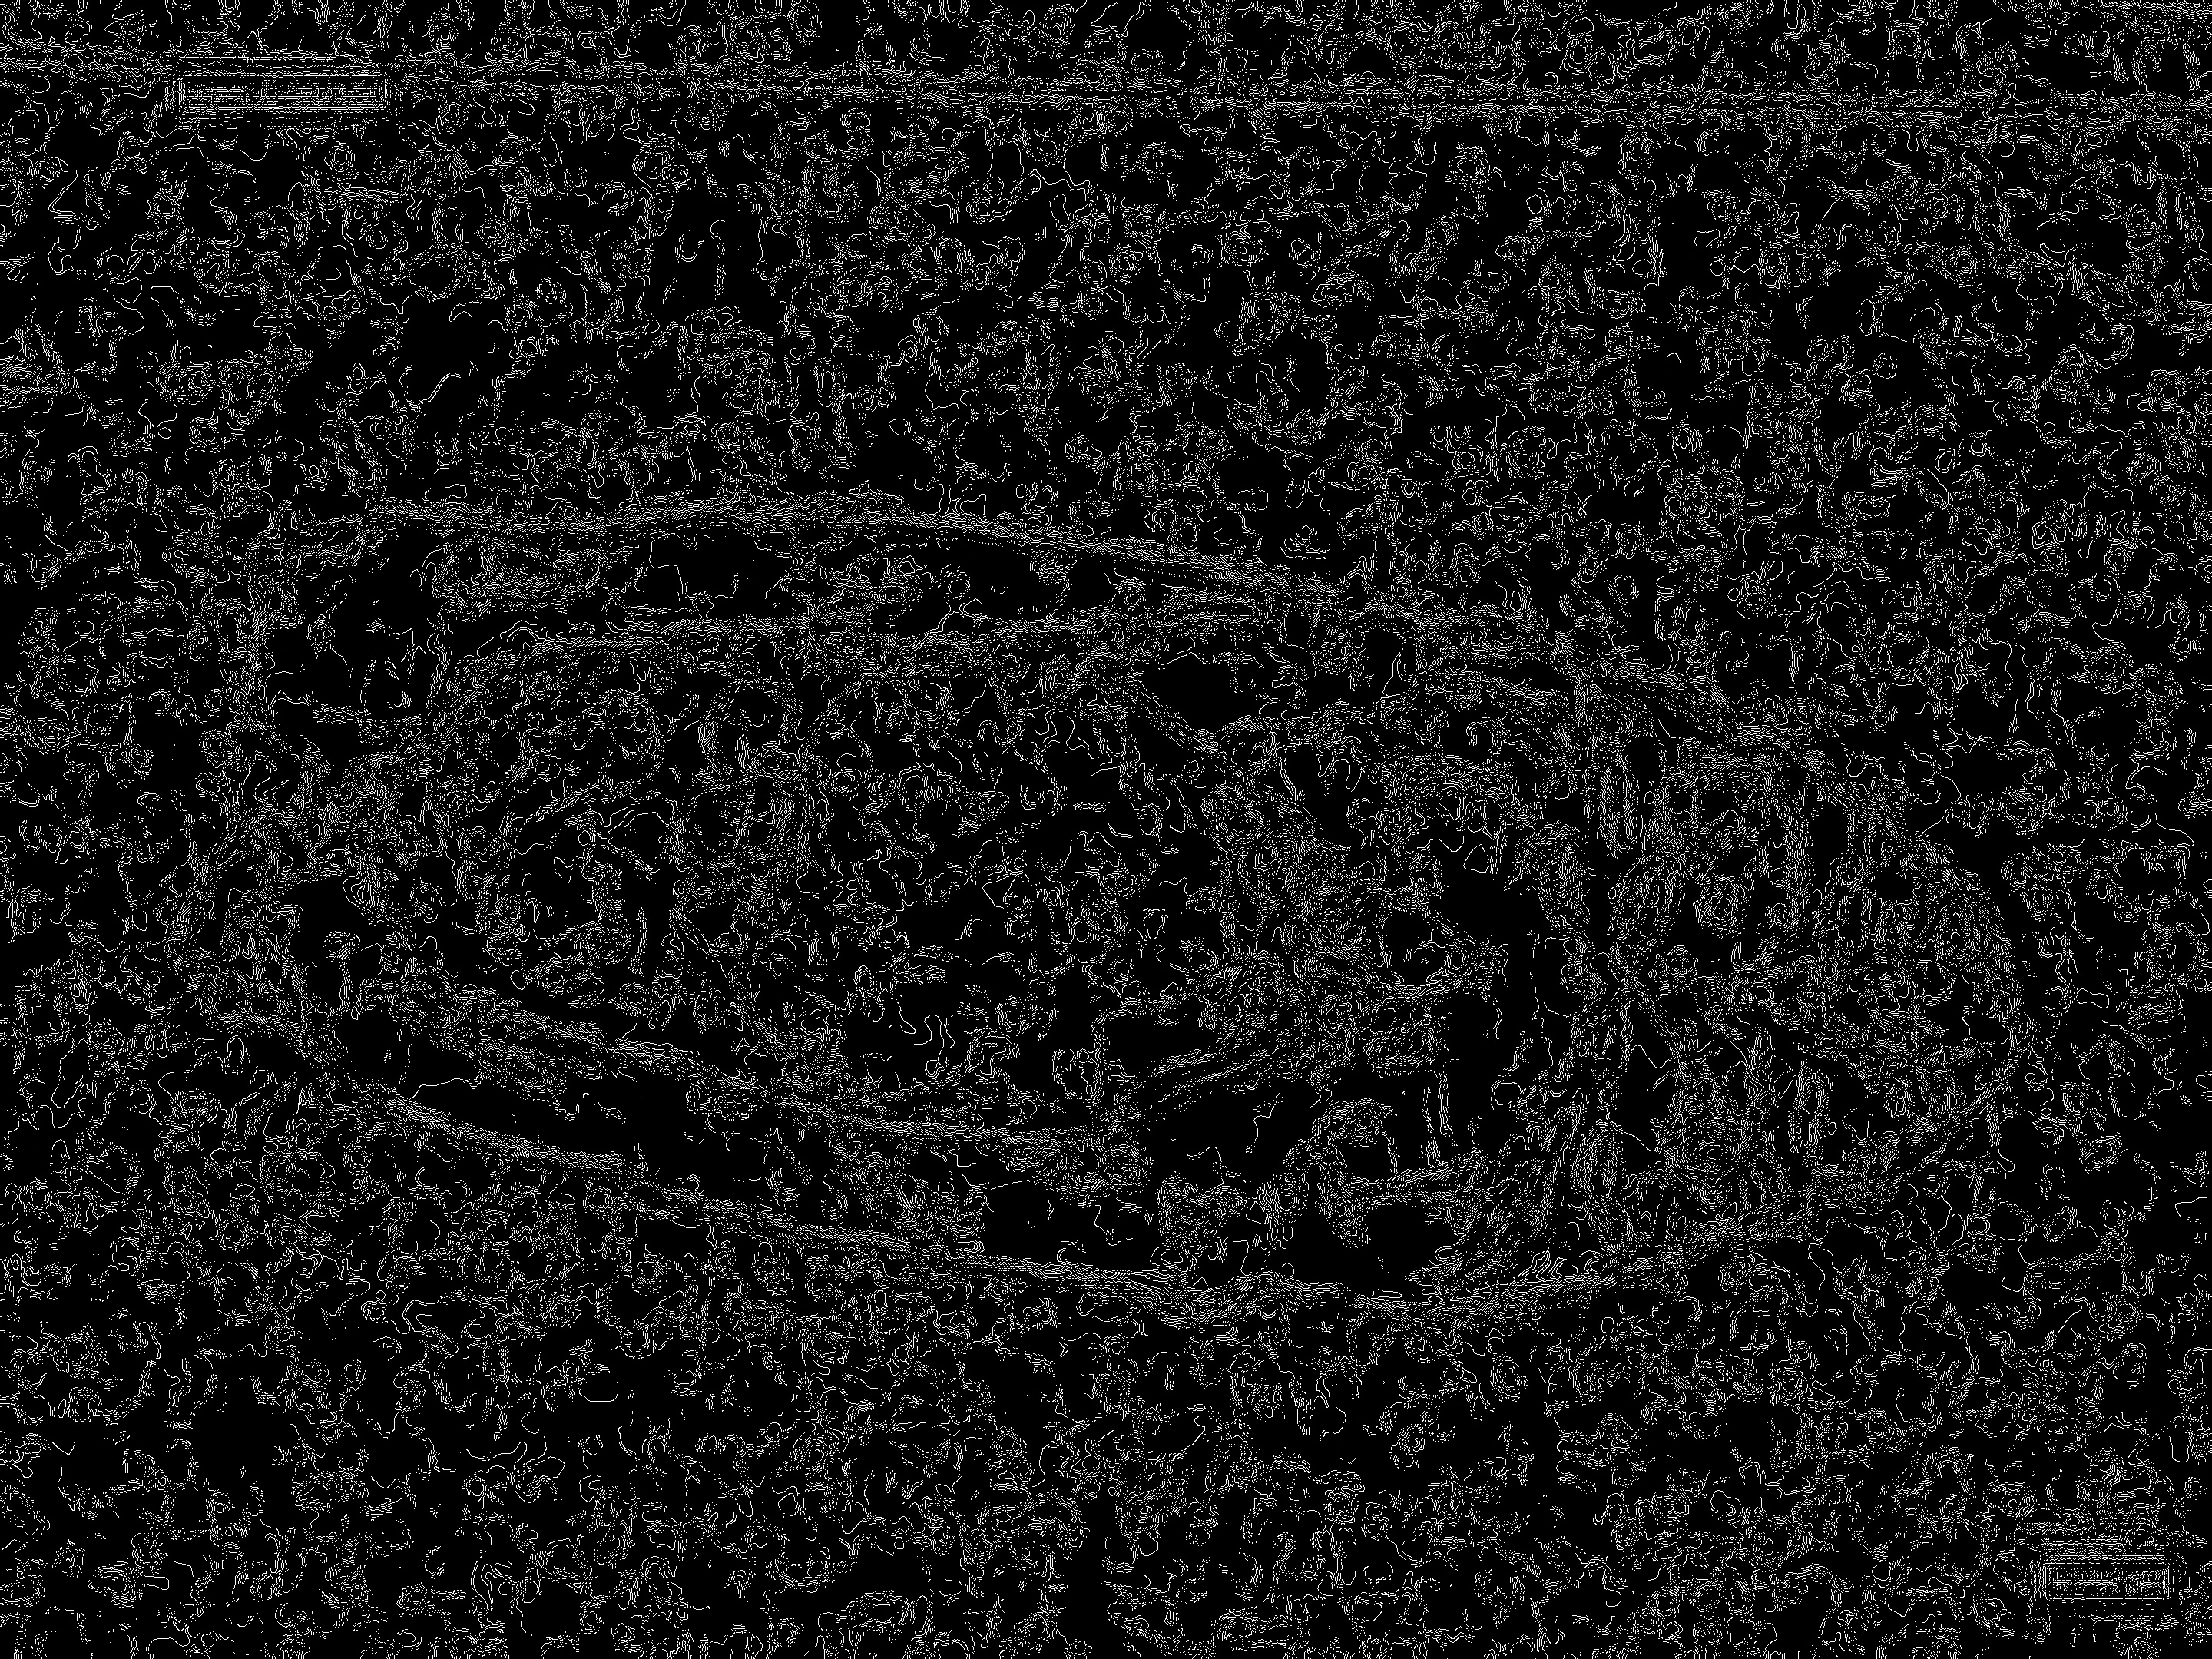
\includegraphics[width=\textwidth]{./fig/gausssian/canny61+2.jpg}
        \caption{canny 2 5}
        \label{fig:canny2_5}
    \end{minipage}
    \begin{minipage}{0.32\textwidth}
        \centering
        \includegraphics[width=\textwidth]{./fig/gausssian/canny61+4.jpg}
        \caption{canny 4 10}
        \label{fig:canny4_10}
    \end{minipage}
    \begin{minipage}{0.32\textwidth}
        \centering
        \includegraphics[width=\textwidth]{./fig/gausssian/canny61+6.jpg}
        \caption{canny 6 15}
        \label{fig:canny6_15}
    \end{minipage}
\end{figure}


在三个Canny结果中,\autoref{fig:canny4_10} 的表现最好,能够保留大部分边缘细节,同时有效地消除了大部分噪声。因此,选择了4和10作为Canny算法的阈值。

\textbf{总结}

比较Sobel、Laplacian和Canny算法的结果,Sobel算法的表现一般,边缘检测明显,但噪声减少有限。Laplacian算法的表现最差,边缘几乎变得不可见,可能是由于其对噪声的高敏感度。Canny算法的结果最好,保持了边缘细节,同时有效地去除了大部分噪声。因此,选择Canny算法作为图像预处理的方法,增强了模型对于进一步分析的相关特征的关注能力。

\subsubsection{Threshold Segmentation}
考虑到生物组织样本(黄色)和标本中的石蜡(白色)的颜色差异,阈值分割提供了一种直接的方法来区分这两个组成部分,通过隔离图像的白色区域,保留生物组织。这个过程包括增强图像的对比度和饱和度,以更好地突出生物组织的黄色,如 \autoref{fig:enhanced_image} 所示。处理步骤使用 Python 的 OpenCV 库执行。

首先,评估图像中的每个像素,保留黄色像素周围大约半径 15(约为图像宽度的 1\%)的像素。其他颜色被移除,如 \autoref{fig:yellowpic} 所示。然而,由于切割过程中组织碎片的分散,这种方法显示出了限制,这些碎片可能散布在整个标本中,干扰了黄色像素的检测。

\begin{figure}[H]
    \centering
    \begin{minipage}{0.45\textwidth}
        \centering
        \includegraphics[width=\textwidth]{./fig/threshold/enhanced_image.jpg}
        \caption{增加对比度}
        \label{fig:enhanced_image}
    \end{minipage}
    \begin{minipage}{0.45\textwidth}
        \centering
        \includegraphics[width=\textwidth]{./fig/threshold/yellowpic.jpg}
        \caption{保留黄色像素}
        \label{fig:yellowpic}
    \end{minipage}
\end{figure}

为了精细化分割,需要进一步处理以消除图像中出现的黑色块。这是通过应用掩码反转来实现的,将这些黑色块变成白色,从而增强了生物组织与石蜡基底的分离。结果显示在 \autoref{fig:mask} 中。

\begin{figure}[H]
    \centering
    \begin{minipage}{0.45\textwidth}
        \centering
        \includegraphics[width=\textwidth]{./fig/threshold/final.jpg}
        \caption{移除黑色块后的最终图像}
        \label{fig:mask}
    \end{minipage}
    \begin{minipage}{0.45\textwidth}
        \centering
        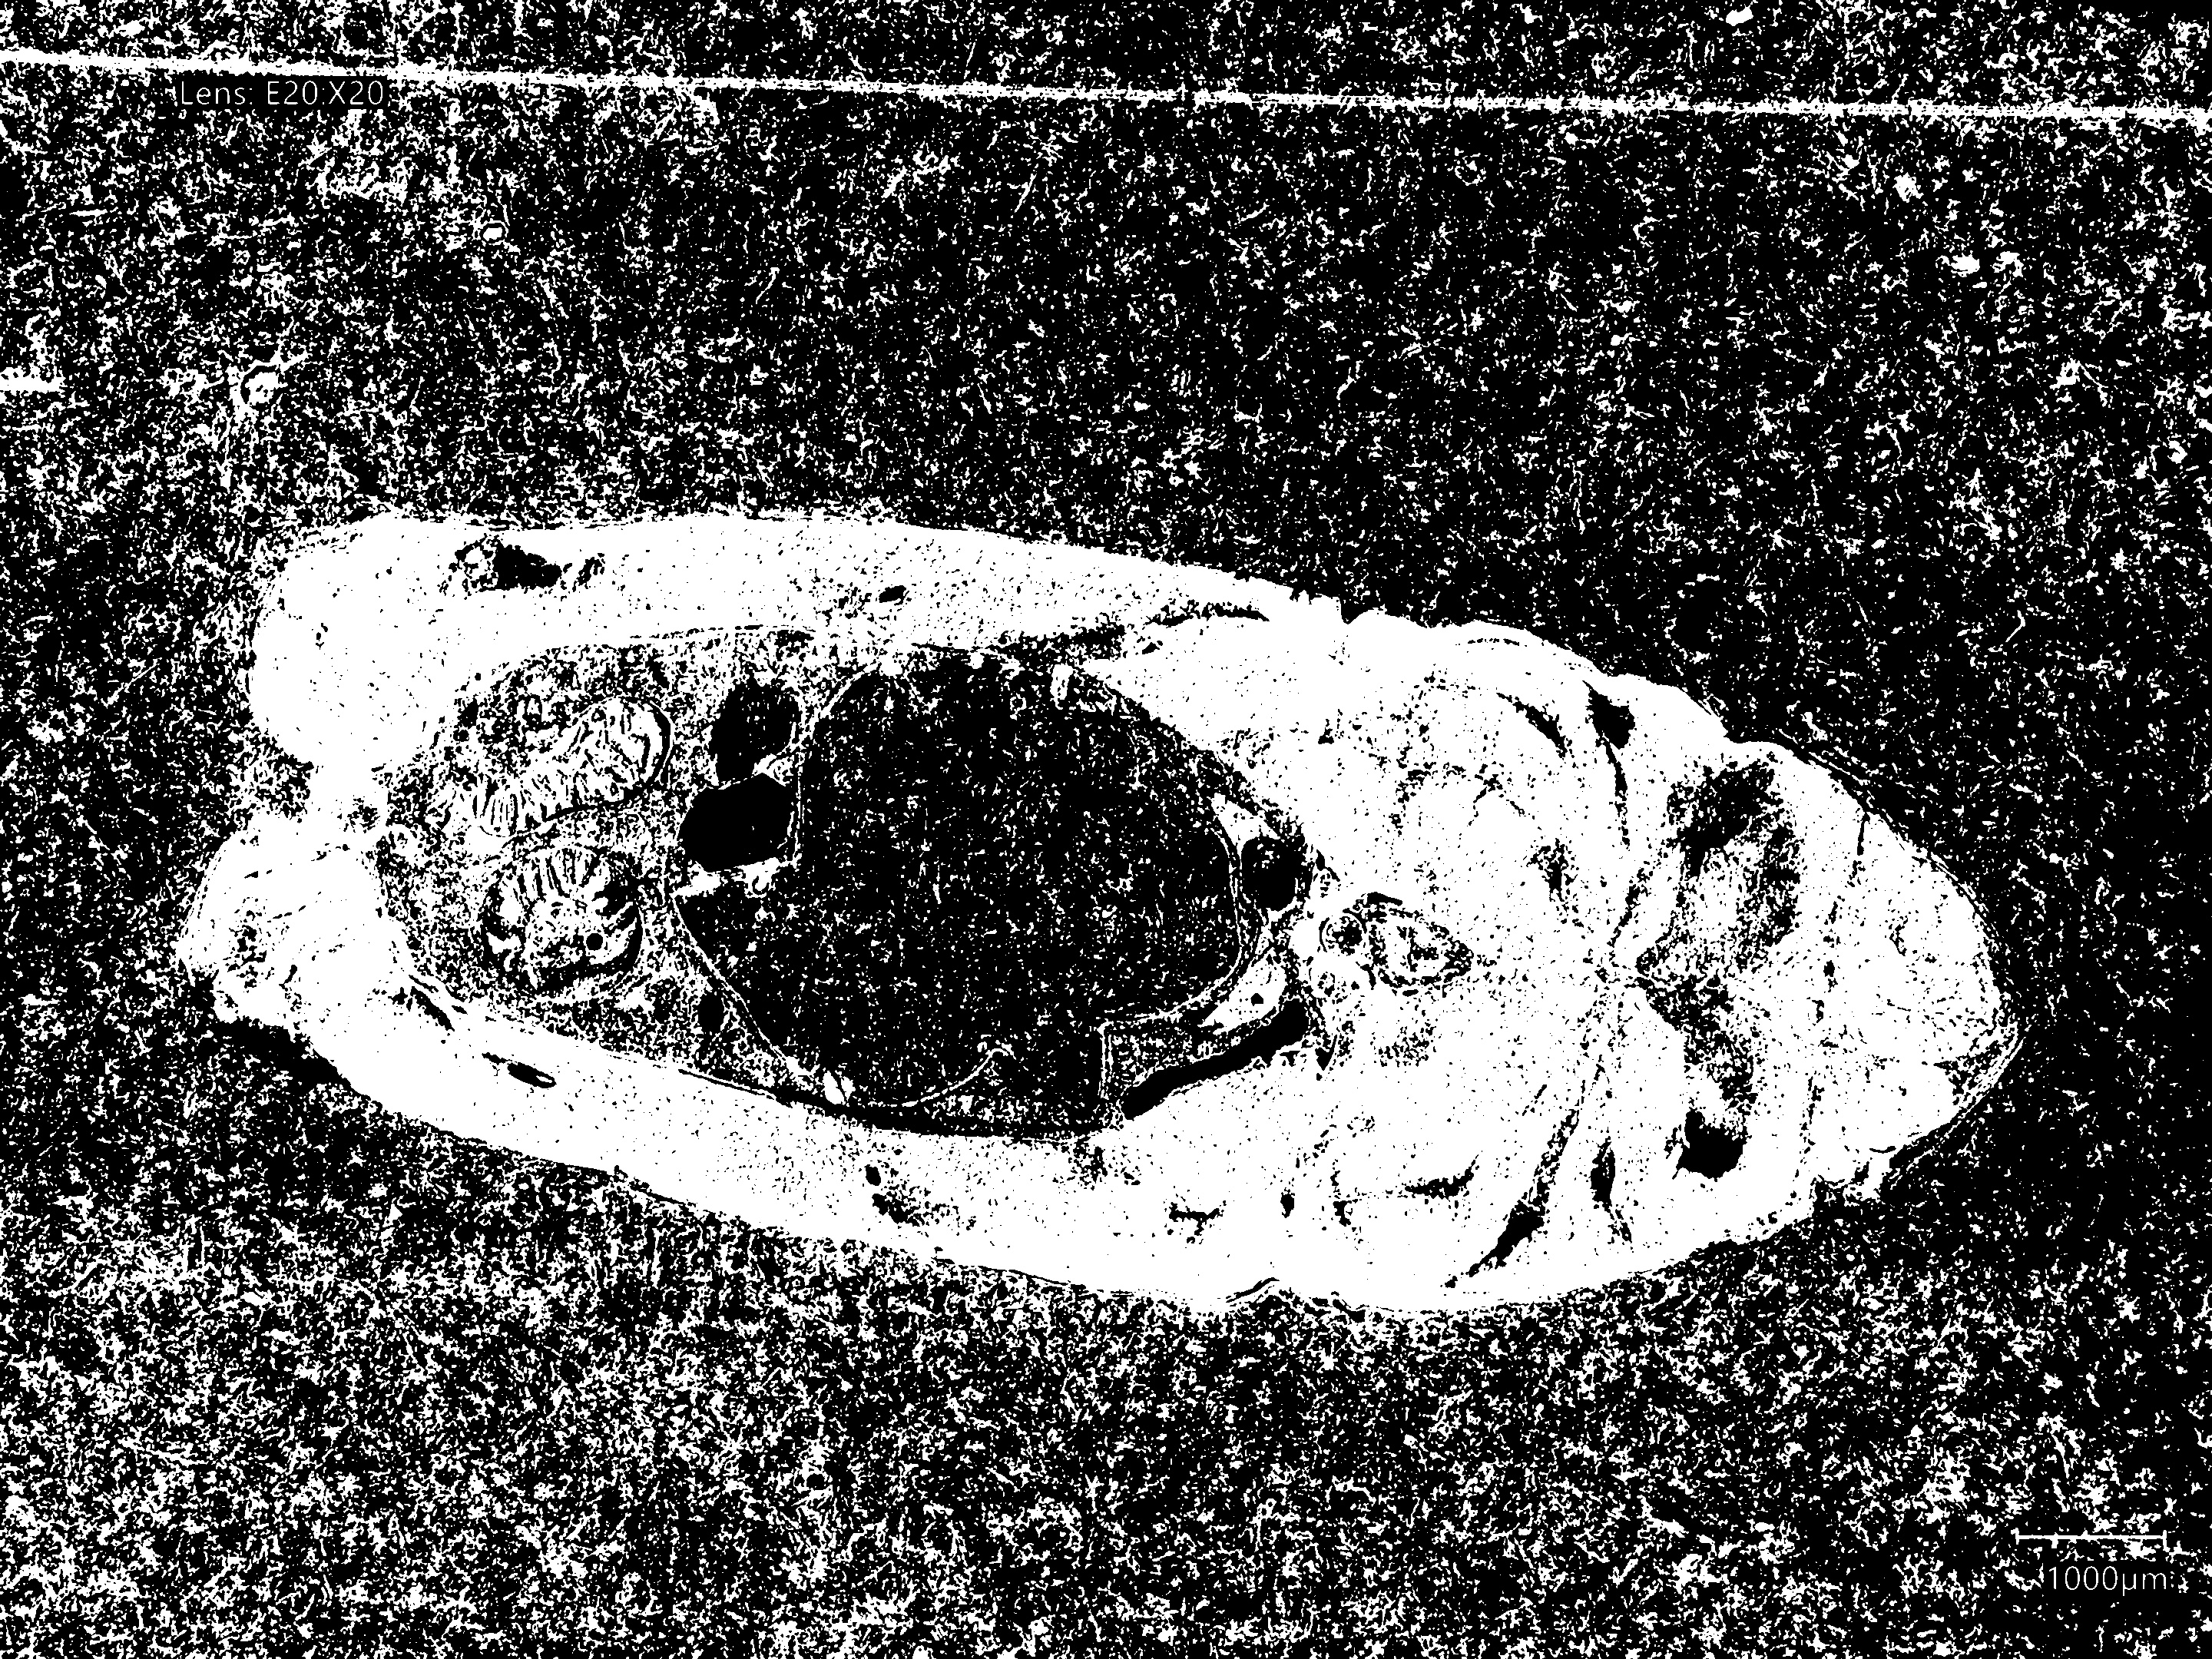
\includegraphics[width=\textwidth]{./fig/threshold/fingerprint.jpg}
        \caption{使用指纹算法进行分割的结果}
        \label{fig:fingerprint}
    \end{minipage}
\end{figure}

这种方法展示了结合颜色增强和阈值分割技术有效地从显微图像中分割生物组织和石蜡的实用性。挑战在于准确地区分组织碎片与背景噪声和其他非组织元素。这种方法对于组织病理学中的自动图像分析特别有效,其中准确的组织分割对于研究至关重要。

\subsubsection{另一种阈值分割方法:指纹算法}
在文献回顾过程中,找到了一篇描述了基于 Otsu 算法的改进分割方法的文章,专门适用于指纹分割。考虑到组织切片和指纹都是具有复杂模式和纹理的生物组织,我们假设这种算法也可能对切片组织的分割有效。应用这种方法的结果在 \autoref{fig:fingerprint} 中进行了说明。

指纹算法是 Otsu 方法的一种改编,特别有效于区分高密度和低密度区域,这对于需要区分脊和谷的对比度的应用,如指纹识别,是理想的。在生物组织分割的背景下使用这种算法可能提供一种强大的方式来划定样本内不同细胞密度或结构的区域。

\subsubsection{总结}

基于讨论的图像预处理技术,边缘检测和阈值分割在突出生物组织的特征和消除石蜡干扰方面都显示出了有希望的结果。这些预处理步骤显著增强了关键特征的可见性,同时最小化了噪声和无关信息,这对于组织病理学中的准确分析至关重要。

为了利用这些改进,可以建立三个数据集:

\begin{itemize}
    \item 通过 \textbf{边缘检测} 处理的图像。
    \item 通过 \textbf{阈值分割} 处理的图像。
    \item 使用 \textbf{指纹算法} 处理的图像。
\end{itemize}

这些数据集将作为即将进行的模型训练阶段的训练集。利用多样的预处理方法不仅增强了模型的鲁棒性,通过提供数据的多样表示,而且有助于探索哪种图像预处理技术最能有效地帮助模型学习相关特征。

\subsection{模型 2:使用简单 CNN 网络的预处理图像}

在本节中,我们将模型 1c(从前面的实验中表现最好的模型)调整为使用预处理图像。架构保持不变;然而,输入现在由经过各种预处理技术的图像组成:

\begin{itemize}
    \item \textbf{模型 2a:} 使用经过 Canny 边缘检测处理的图像。
    \item \textbf{模型 2b:} 使用经过阈值分割处理的图像。
    \item \textbf{模型 2c:} 输入是使用指纹算法分割的图像。
\end{itemize}

每个模型都遵循模型 1c 的架构,包括每个具有 32 个特征图和 3x3 内核的三个卷积层,最大池化层,以及一个具有 256 个神经元的全连接层。

结果显示在下面的图中(\autoref{fig:model22_acc} 和 \autoref{fig:model22_loss}),展示了模型 2a、2b 和 2c 的训练和验证准确率以及损失。
\begin{figure}
    \centering
    \begin{minipage}{0.49\textwidth}
        \centering
        \includegraphics[width=\textwidth]{./fig/model2/accuracy22.eps}
        \caption{模型 2 的准确率}
        \label{fig:model22_acc}
    \end{minipage}
    \begin{minipage}{0.49\textwidth}
        \centering
        \includegraphics[width=\textwidth]{./fig/model2/loss22.eps}
        \caption{模型 2 的损失}
        \label{fig:model22_loss}
    \end{minipage}
\end{figure}


\subsubsection{小结}
图表显示,模型 2a 和 2c 在大约 8 个训练周期后开始稳定,训练准确率接近 100\%,而验证准确率分别稳定在 65\% 和 75\% 左右。尽管准确率高,但这两个模型的验证损失都相对较高,超过 1,这表明过拟合和对未见过的数据的泛化能力有限。

然而,模型 2b 在大约 10 个训练周期后收敛,显示出最高的验证准确率,约为 82\%,并且损失在 1 和 1.2 之间波动。这表明模型 2b 在验证集上的表现更好,表明更好的适应性和鲁棒性。这可能是因为模型 2b 处理的是彩色图像,这些图像从 RGB 通道提供了更丰富的特征,可能增强了特征提取和泛化能力。

然而,有一种风险是在预处理步骤中可能会丢失重要的细节,特别是在模型 2b 的阈值分割中。这可能会对模型在特定类型的图像上的性能产生负面影响。以下是这种关键信息丢失的一个例子:

\begin{figure}
    \centering
    \begin{minipage}{0.45\textwidth}
        \centering
        \includegraphics[width=\textwidth]{./fig/model2/origin20240205_161427.jpg}
        \caption{原始图像}
        \label{fig:origin}
    \end{minipage}
    \begin{minipage}{0.45\textwidth}
        \centering
        \includegraphics[width=\textwidth]{./fig/model2/yellow20240205_161427.jpg}
        \caption{阈值分割}
        \label{fig:yellow}
    \end{minipage}
\end{figure}

在 \autoref{fig:yellow} 中,我们看到模型 2b 的训练集中使用的阈值分割算法显著增强了水平褶皱,可能在训练过程中使模型混淆。

这些发现突显了图像预处理的挑战。过度的预处理有时会消除关键信息,导致训练结果降低。在未来的步骤中,可能会采用迁移学习,使用适应我们数据集的预训练的大规模深度学习模型,以提高训练效果并解决这些挑战。

\subsection{模型 3:原始图像与迁移学习}

\textbf{使用预训练模型的迁移学习}

我们正在整合三个在 ImageNet 数据集上预训练的知名模型:VGG16、VGG19 和 InceptionV3。这些模型带有预训练的权重,这些权重经过高度优化,预计在适应我们特定的数据集时,将显著提高特征提取能力。

\begin{itemize}
    \item VGG16(模型 3a)和 VGG19(模型 3b)相似,但 VGG19 有三个额外的卷积层,可能提供更好的特征提取能力。
    \item InceptionV3(模型 3c)整合了 Inception 模块,使其能够在多个尺度上捕获更广泛的特征,提供更复杂且可能更有效的特征提取机制。
\end{itemize}

\textbf{迁移学习的适应性}

为了防止过拟合并优化迁移学习过程:

\begin{itemize}
    \item 使用了早停法。
    \item 学习率设定较低,对于 VGG16 和 VGG19 为 1e-5,对于参数更少的 InceptionV3 稍高,为 1e-4。
    \item 所有模型都被调整为接受 224x224 的输入大小,除了 InceptionV3 使用其默认的输入大小 299x299。这种统一的输入大小有助于标准化数据预处理步骤。
    \item 在每个模型的基础模型层之后添加了一个全局平均池化层,然后是一个与输出类别数匹配的全连接层。
\end{itemize}

\textbf{模型训练的观察}

以下是这些模型的训练和验证性能:

\begin{figure}[H]
    \centering
    \begin{minipage}{0.49\textwidth}
        \centering
        \includegraphics[width=\textwidth]{./fig/model3/accuracy33.eps}
        \caption{模型 3 的准确率}
        \label{fig:model33_acc}
    \end{minipage}
    \begin{minipage}{0.49\textwidth}
        \centering
        \includegraphics[width=\textwidth]{./fig/model3/loss33.eps}
        \caption{模型 3 的损失}
        \label{fig:model33_loss}
    \end{minipage}
\end{figure}

\textbf{分析}
\begin{itemize}
    \item 模型 3b(VGG19)和 3c(InceptionV3)显示出约 90\% 的显著更高的验证准确率,与模型 3a(VGG16)相比。
    \item 损失指标表明,模型 3c(InceptionV3)在三者中具有最低的验证损失,表明它在泛化到未见过的数据方面最为有效。这突显了 InceptionV3 在捕获复杂特征方面的优越能力。
    \item 模型 3a 和模型 3b 之间的性能差距支持了这样的观点,即 VGG19 中额外的卷积层增强了其比 VGG16 更有效地处理图像特征的能力。
\end{itemize}

\subsubsection{小结}

对 VGG16、VGG19 和 InceptionV3 模型的比较分析显示,InceptionV3 提供了最佳的训练结果,其训练和验证准确率分别收敛于 1 和 0.9 左右,损失收敛于 0.6。这表明 InceptionV3 模型不仅有效地进行训练,而且展示了优越的泛化能力。

\subsection{模型选择总结}
当在模型系列——模型 1、模型 2 和模型 3——之间进行比较时,显然模型 3 的表现最好,特别是模型 3c。其根本原因可能是由于模型 3 基于在大规模图像数据集上预训练的深度卷积网络,使得特征提取更有效,能够开发出强大的特征空间。

\textbf{模型 3c(InceptionV3)的显著特性:}

\begin{itemize}
    \item \textbf{架构设计:} InceptionV3 具有模块化设计,包含多个 "inception 模块",这些模块包括在同一层内并行操作的多尺度卷积层。这种模块化方法使网络能够在各种尺度和深度上捕获广泛的特征。
    \item \textbf{特征提取:} Inception 模块可以通过在同一层内处理不同尺度的特征来适应性地捕获适当的特征表示。这种适应性使其特别适合处理复杂的图像数据,如生物医学图像。
    \item \textbf{深度网络处理:} InceptionV3 集成了批量归一化和残差连接,这些在训练深度网络中至关重要。这些技术有效地缓解了梯度消失的问题,从而有助于训练更深的模型而不降低性能。
\end{itemize}

考虑到这些优点,模型 3c(InceptionV3)被选为我们的最终模型,用于进一步的应用和测试。这个模型不仅因其先进的架构创新而突出,而且因其在泛化到新的、未见过的数据方面的证明效果而突出,使其非常适合复杂的任务,如医学图像分析,其中准确性和可靠性至关重要。

% \section{Discussion and conclusions}
\subsection{Subsection 3.1}

\subsection{Subsection 3.2}

% \section{Discussion and conclusions}
\label{sec:results}

\subsection{讨论}

\subsection{总结}


\subsection{提升和改进}








\FloatBarrier % Now the table doesn't flow over to any other sections

% %Conclusion


%%-----------English
\pagenumbering{arabic}
\section{Introduction and background}
\label{sec:introduction}
\subsection{Background}

As the fundamental units of life, human research into cells and tissues has never ceased. Biological tissue sections, serving as crucial means for the direct observation of cellular morphology and structure, are essential for biomedical research and clinical diagnosis. A complete and usable tissue section is of great importance to researchers and physicians, as it provides vital information about cell structure, tissue morphology, and pathological changes. Within this, the quality of the section is of paramount importance.

Traditional manual sectioning methods are time-consuming and prone to variability, hence the emergence of automatic microtomes has provided a solution to these issues. For different biological tissues, varying cutting parameters can yield differing results, both positive and negative. Therefore, to enhance the utilization rate of biological sections and increase the production of high-quality specimens, determining optimal cutting parameters for specific tissues remains a goal.

Machine learning and deep learning have achieved significant success in the fields of computer vision and image processing. Machine learning is defined as a series of methods that can automatically detect patterns in data, which are then used to predict future outcomes or make decisions \cite{1.1}. In this paper, we integrate advanced image analysis and machine learning techniques to identify section quality and then evaluate the quality of tissue samples under different sectioning parameters.

\subsection{Introduction}
\textbf{Project Overview}

This project aims to optimize the cutting parameters of biological tissue microtomes, which are crucial devices in biomedical research and clinical diagnostics. The objective is to enhance the precision and efficiency of tissue sample preparation by determining the optimal slicing conditions. By collecting tissue samples under various cutting parameters and conducting subsequent manual image classification, this study employs deep learning techniques to analyze and predict the most effective cutting parameters. This work not only promises to improve the quality of tissue samples for microscopic examination but also helps to simplify laboratory workflows, thereby advancing biological and medical sciences.

\textbf{Objectives:}

\begin{enumerate}
    \item Collect a comprehensive dataset of tissue samples sliced under different parameters.
    \item Employ artificial image classification to categorize the quality and characteristics of these samples.
    \item Develop and train a deep learning model capable of assessing tissue sample quality.
    \item Use the model's insights to determine the optimal cutting parameters for the tissue slicer.
    \item Validate the model's predictions through empirical testing and refinement.
\end{enumerate}


\subsection{Structure of the Report}
The report is organized into multiple chapters, each focusing on specific aspects of the research on optimizing biopsy parameters using deep learning:

\textbf{Introduction and Background} - This initial chapter outlines the project's goals and framework, provides the motivation for the research, and describes the technical protocols and standards employed.

\textbf{Literature Review} - An extensive review of the relevant literature on biological tissue sections, image classification, and deep learning applications in biological sample preparation. This section contextualizes the current study within existing research.

\textbf{Methods and Theory} - A comprehensive description of the experimental methods, theoretical frameworks, and plans for data collection and processing.

\textbf{Experimental Work/Analysis Investigation/Design} - Details the experimental design, implementation, and analytical survey, explaining the strategies and methods used to meet the project objectives.

\textbf{Presentation of Experimental or Analysis Results/Final Constructed Product Description} - This chapter documents the experimental data, analysis results, or descriptions of the final design products, elaborating on the outcomes.

\textbf{Discussion and Conclusion} - Discusses the results in terms of their scientific significance and practical implications, draws conclusions, and suggests future research directions.

\textbf{Project Management, Sustainability, and Health Safety Considerations} - Covers project management strategies, addresses sustainability and health safety issues to ensure the research is conducted efficiently and safely.

\textbf{References} - Compiles all literature referenced throughout the research, supporting the study's foundation.


\textbf{Assumptions and Technical Specifications} - The project relies on several assumptions:

\begin{enumerate}
    \item Uniform properties of tissue samples across different batches.
    \item Reliability and accuracy of the biological tissue microtome and imaging equipment.
    \item Effectiveness of deep learning models in interpreting complex biological image data.
\end{enumerate}

Technical details regarding tissue microtome settings, image classification standards, and deep learning architecture are thoroughly described in the Methods and Theory section.

\section{Literature review}

This literature review explores the integration of technologies in biological tissue sectioning, with a particular focus on the application of image classification and deep learning in optimizing slicing parameters. It aims to highlight significant advancements, identify gaps in current methodologies, and lay the groundwork for the proposed project.

\subsection{Microtome and Microscope}

In recent years, the advent of automatic microtomes has significantly simplified the sectioning process and improved the quality of sections.

Zimmermann, in the article "Improved reproducibility in preparing precision-cut liver tissue slices," advocates for the use of the new Leica vibratome to enhance the accuracy and reproducibility of tissue sections from rats, mice, and human tissues \cite{LR.1}.

In this experiment, the HM355S microtome provided by Epredia is used for sectioning. This machine is a popular device for biological tissue sectioning research, and many experiments and papers have utilized this equipment for sectioning.

Elzbieta Klimuszko has used the HM355S microtome for sectioning teeth to investigate the calcium and magnesium content in dental enamel \cite{LR.2}.

Andelko Hrzenjak also used the HM355S microtome for sectioning pathological endometrial tissues to study the mechanisms of endometrial carcinoma development \cite{LR.3}.

Similarly, the choice of microscope is crucial. In this experiment, the VHX7000 microscope from Keyence is used for image acquisition. It is capable of capturing images of biological tissue sections (e.g., mouse prostate cells \cite{LR.4}),
as well as inorganic materials (such as ceramics \cite{LR.5}, glass \cite{LR.6}).

The experiments will employ the HM355s microtome and VHX7000 microscope for sectioning and image acquisition. This setup ensures that both equipment selection and technological application are optimally aligned to enhance the precision and efficiency of the tissue sectioning process, supporting the overall goals of the research project.

% 近年来,自动切片机的出现显著简化了切片过程,并提高了切片的质量。

% Zimmermann在文章"Improved reproducibility in preparing precision-cut liver tissue slices"中,主张使用新的Leica振动刀来提高大鼠、小鼠和人体组织切片的精度和重复性 \cite{LR.1}。

% 在这个实验中,我们使用Epredia提供的HM355S切片机进行切片。这台机器是生物组织切片研究的流行设备,许多实验和论文都使用了这台设备进行切片。

% Elzbieta Klimuszko使用HM355S切片机切割牙齿,以研究牙釉质中的钙和镁含量 \cite{LR.2}。

% Andelko Hrzenjak也使用HM355S切片机切割病理性子宫内膜组织,以研究子宫内膜癌发展的机制 \cite{LR.3}。

% 同样,显微镜的选择也至关重要。在这个实验中,我们使用Keyence的VHX7000显微镜进行图像采集。它能够捕获生物组织切片的图像(例如,小鼠前列腺细胞 \cite{LR.4}),以及无机材料(如陶瓷 \cite{LR.5},玻璃 \cite{LR.6})。

% 实验将使用HM355s切片机和VHX7000显微镜进行切片和图像采集。这种设置确保了设备选择和技术应用的最佳配合,以提高组织切片过程的精度和效率,支持研究项目的总体目标。

\subsection{Deep Learning in Tissue Sectioning}

The application of deep learning technologies in the biomedical field has achieved significant advancements. Deep learning models excel in tasks such as image classification, object detection, and segmentation, providing powerful tools for research and diagnostics in biomedical laboratories.

Lorena Guachi-Guachi proposed a method utilizing CNN networks to identify and refine tissue sections. This approach represents an innovative application of deep learning that can enhance the precision of tissue preparation and analysis \cite{LR.7}.

In the book \textit{Biomedical Texture Analysis}, Vincent Andrearczyk introduced a CNN architecture specifically designed for texture analysis, which significantly improves the accuracy of classifying biological tissues compared to traditional architectures \cite{LR.8}. This development demonstrates the potential of deep learning to enhance the detailed analysis of tissue characteristics, which is crucial for accurate diagnostics and research.

Yan Xu suggested that features extracted from CNNs trained on the large natural image database, ImageNet, can be transferred to histopathological images of tissues. This provides a viable approach for implementing transfer learning, which can greatly enhance the efficiency of tissue image classification and analysis \cite{LR.9}.

Based on the literature, deep learning technology holds broad prospects for application in image classification and analysis of tissue sections. By leveraging deep learning models, efficient identification and classification of tissue samples can be achieved, providing strong support for optimizing sectioning parameters.

This section underscores the transformative impact of deep learning on the field of tissue sectioning, promising significant improvements in the accuracy and utility of histological analyses.

% 在生物医学领域,深度学习技术的应用已取得了显著的进步。深度学习模型在图像分类、对象检测和分割等任务中表现出色,为生物医学实验室的研究和诊断提供了强大的工具。

% Lorena Guachi-Guachi 提出了一种利用 CNN 网络识别和精炼组织切片的方法。这种方法代表了深度学习的创新应用,可以提高组织准备和分析的精度 \cite{LR.7}。

% 在《生物医学纹理分析》一书中,Vincent Andrearczyk 介绍了一种专为纹理分析设计的 CNN 架构,与传统架构相比,这种架构显著提高了生物组织分类的准确性 \cite{LR.8}。这一发展展示了深度学习提高组织特性详细分析的潜力,这对于准确的诊断和研究至关重要。

% Yan Xu 提出,从在大型自然图像数据库 ImageNet 上训练的 CNN 中提取的特征可以转移到组织的病理学图像上。这为实施转移学习提供了一种可行的方法,可以大大提高组织图像分类和分析的效率 \cite{LR.9}。

% 根据文献,深度学习技术在组织切片的图像分类和分析中有广阔的应用前景。通过利用深度学习模型,可以实现组织样本的有效识别和分类,为优化切片参数提供了强大的支持。

% 这一部分强调了深度学习对组织切片领域的变革性影响,预示着在组织学分析的准确性和实用性方面的显著改进。



\section{Methodology and theory}
\label{sec:problem_description}

\subsection{Computer Vision - Image Segmentation}

For the acquired image data, appropriate image preprocessing can be applied. Under the premise of maintaining the integrity and quality of images, certain processing can be implemented to highlight the features intended for computer recognition and, to some extent, remove irrelevant features and noise. This enhances the accuracy of subsequent deep learning models.

Image segmentation is a critical step in image processing, aiming to divide the image into several meaningful regions for further analysis and processing. In models focusing on the yield rate of biological tissues, it is necessary to segment the biological sections into biological tissue and paraffin areas, emphasizing the biological tissue parts.

Common image segmentation algorithms include edge detection and threshold segmentation.

\subsubsection{Edge Detection}
For biological tissue sections, a crucial indicator of quality is the clarity of the section's edges. The integrity and continuity of the slice edges can reflect whether there are quality issues with the sample.

There are numerous algorithms for edge detection, such as Sobel, Laplacian, and Canny operators \cite{3.1}.

The \textbf{Sobel operator} is a first-order differential operator that can be used to detect image edges \cite{补充1}. Suppose there is a one-dimensional image $f(x)$, the relationship between its intensity and the pixel coordinate $x$ can be represented as shown in Figure 1. It can be observed in \autoref{fig:original_function} that the slope is the largest around x=2.2, indicating that there is a sudden change in image intensity (an edge exists) near this point. Taking its derivative gives the first-order derivative $f'(x)$, as shown in \autoref{fig:first_derivative}, where the absolute value of the derivative is the largest. The Sobel operator uses this characteristic to detect edges.

\begin{figure}[htbp]
    \centering
    \begin{minipage}[b]{0.32\textwidth}
        \centering
        \includegraphics[width=\textwidth]{./fig/original_function.png}
        \caption{f(x)}
        \label{fig:original_function}
    \end{minipage}
    \begin{minipage}[b]{0.32\textwidth}
        \centering
        \includegraphics[width=\textwidth]{./fig/first_derivative.png}
        \caption{f'(x)}
        \label{fig:first_derivative}
    \end{minipage}
    \begin{minipage}[b]{0.32\textwidth}
        \centering
        \includegraphics[width=\textwidth]{./fig/second_derivative.png}
        \caption{f''(x)}
        \label{fig:second_derivative}
    \end{minipage}
\end{figure}

The \textbf{Laplacian operator} is a second-order differential operator that performs well in edge detection of images. It is derived by taking the derivative of the Sobel operator once more. In 2D images, the Laplacian operator is defined as follows: 

\begin{equation} 
    \nabla^2 f = \frac{\partial^2 f}{\partial x^2} + \frac{\partial^2 f}{\partial y^2} 
\end{equation} 

As shown in the figure above, taking the derivative of the first-order derivative results in the second-order derivative $f''(x)$, as shown in \autoref{fig:second_derivative}. It can be seen that around x=2.2, the second-order derivative is 0, which indicates that when the value of the Laplacian operator $\nabla^2 f$ is 0, there is a sudden change in image intensity, indicating the presence of an edge.

\textbf{Canny Operator}is a multi-stage differential operator that enhances the edge detection process by incorporating noise suppression, building on the initial computations similar to those used by the Sobel operator. Introduced by John F. Canny in 1986 \cite{3.2}, the Canny operator refines the results obtained from Sobel operator calculations through additional steps such as non-maximum suppression and hysteresis thresholding. These steps set thresholds to eliminate false edges from the image, resulting in more accurate edge detection.

In the chapter on \textit{Experimental Work/Analytical Investigation/Design}, experiments will be conducted on the collected image data using these three edge detection algorithms—Sobel, Laplacian, and Canny—to compare their effectiveness. This comparative analysis will help in identifying the most suitable method for edge detection in the context of tissue sectioning, where the clarity and precision of edges are vital for quality assessment. The results will guide the selection of the optimal algorithm to be integrated into the image processing pipeline, enhancing the capability of the system to accurately segment and analyze biological tissue sections.

\subsubsection{Theresold Segmentation}

Apart from edge detection, another method employed is threshold segmentation. This technique divides the image pixels into two categories: those above a certain threshold and those below it. It is particularly useful in situations where there is a significant grayscale difference between the target and the background in the image.

For specimens, a straightforward approach is to contrast the colors of the paraffin area and the biological tissue area (which is stained during preparation), and then separate them using threshold segmentation. Assuming the biological tissue is yellow and the paraffin is white, setting a threshold could isolate the white parts of the image, leaving behind the biological tissue.

Additionally, there are more sophisticated methods of threshold segmentation, such as the Otsu method used for fingerprint extraction. Implementing this method can significantly enhance the segmentation of biological tissues. Yue Yaru and Zhu Jialin in "Algorithm of fingerprint extraction and implementation based on OpenCV" have proposed an improved Otsu-based fingerprint extraction algorithm using OpenCV. This algorithm excels particularly under conditions of uneven illumination and blurred images, providing accurate, simple, and fast fingerprint extraction \cite{3.3}.

Comparisons and experiments related to these segmentation techniques will be conducted in the \textit{Experimental Work/Analytical Investigation/Design} chapter.









 
\section{Experimental work/ analytical investigation/ design}

\textbf{Experimental workflow}

The experiment workflow is outlined in the diagram below, detailing the sequential steps from data collection to iterative improvement of the model.

\begin{center}

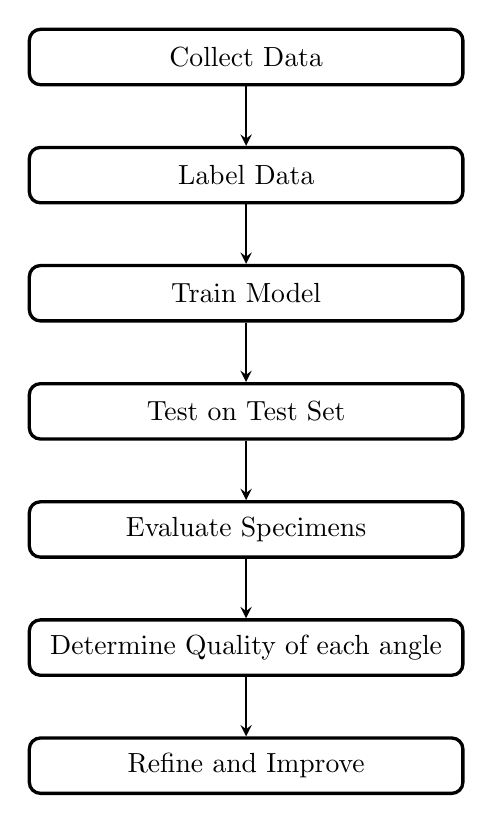
\begin{tikzpicture}[node distance=1.5cm,
    box/.style={
        rectangle,
        rounded corners,
        draw=black, very thick,
        text width=15em,
        minimum height=2em,
        text centered},
    arrow/.style={
        thick,
        ->,
        >=stealth}
    ]

    \node (collect) [box] {Collect Data};
    \node (mix) [box, below of=collect] {Label Data};
    \node (train) [box, below of=mix] {Train Model};
    \node (test) [box, below of=train] {Test on Test Set};
    \node (evaluate) [box, below of=test] {Evaluate Specimens};
    \node (rate) [box, below of=evaluate] {Determine Quality of each angle};
    \node (improve) [box, below of=rate] {Refine and Improve};
    
    \draw [arrow] (collect) -- (mix);
    \draw [arrow] (mix) -- (train);
    \draw [arrow] (train) -- (test);
    \draw [arrow] (test) -- (evaluate);
    \draw [arrow] (evaluate) -- (rate);
    \draw [arrow] (rate) -- (improve);
    
    \end{tikzpicture}
\end{center}



\subsection{Data collection}
The first essential step for deep learning is data collection. In this experiment, pre-prepared paraffin-embedded tissue sections (fish ovary tissues) were used. These sections were placed on an HM355s automatic microtome, and slicing operations were performed according to different cutting angles as specified in the microtome's manual. The cutting data was recorded meticulously.

%在这不要提三个点的鱼的肺泡组织,在后面作为模型二次验证和增强使用。

The schematic diagram of the microtome (taking a tooth as an example) is shown in \autoref{fig:cutting_machine} \cite{4.1}.

\begin{figure}[htbp]
    \centering
    \begin{minipage}{0.48\textwidth}
        \centering
        \includegraphics[width=\textwidth]{./fig/machine.jpg}
        \caption{Microtome}
        \label{fig:machine}
    \end{minipage}
    \begin{minipage}{0.48\textwidth}
        \centering
        \includegraphics[width=\textwidth]{./fig/10266_2018_353_Fig1_HTML.jpg}
        \caption{Working principle of the microtome}
        \label{fig:cutting_machine}
    \end{minipage}
\end{figure}
% https://link.springer.com/article/10.1007/s10266-018-0353-6



% 在切削过程中,从切角为8度开始(如\autoref{fig:machine}中的angle of inclination),每次增加0.5度,直到切角为12度。切片机在切片过程中保持给进速度为25,厚度为1。

In the experiment, the microtome was configured with the following parameters: the mode was set to continuous, the feed rate was 5.0, the trimming value was 25, the speed was set at 32, the water flow rate was 7.5, and the water temperature was approximately 36 degrees Celsius. The cutting angle was adjusted between 8 to 12 degrees.

The biological tissues used for sectioning are shown in Figure \ref{label:sample}. After sectioning, the different types of tissue sections were placed on slides as depicted in Figure \ref{fig:采集样本}. Once dried, these slides were transferred under a VHX7000 microscope for imaging. Each sample was photographed under the microscope to capture electronic image data, as shown in Figure \ref{fig:显微镜}.

\begin{figure}[htbp]
    \centering
    \begin{minipage}{0.3\textwidth}
        \centering
        \includegraphics[width=\textwidth]{./fig/sample.jpg}
        \caption{Biological tissues}
        \label{label:sample}
    \end{minipage}
    \begin{minipage}{0.3\textwidth}
        \centering
        \includegraphics[width=\textwidth]{./fig/采集样本.jpg}
        \caption{Collecting samples}
        \label{fig:采集样本}
    \end{minipage}
    \begin{minipage}{0.35\textwidth}
        \centering
        \includegraphics[width=\textwidth]{./fig/显微镜.jpg}
        \caption{Microscope}
        \label{fig:显微镜}
    \end{minipage}
\end{figure}


Based on this, several hundred images were obtained, each with a resolution of 2880*2160. An example of the samples is shown in \autoref{fig:sample9.5}.


\begin{figure}
    \centering
    \includegraphics[width=0.8\textwidth]{./fig/sample9.5.jpg}
    \caption{Sample with a cutting angle of 9.5 degrees}
    \label{fig:sample9.5}
\end{figure}


\subsection{Data labeling}

For this experiment, the dataset is re-labeled based on the quality of the tissue sections. Overall, the quality of the biological tissues is categorized into two primary classes: normal and bad. Further analysis of the collected data revealed common flaws - the presence of vertical or horizontal white creases on the sections, which clearly indicate unusable slices. Given the distinct nature of these flaws, they are classified into two additional specific categories: \textbf{horizontal line}(\autoref{fig:horizental_line}) and \textbf{vertical line}(\autoref{fig:vertical_line}).

\begin{figure}[H]
    \centering
    \begin{minipage}{0.45\textwidth}
        \centering
        \includegraphics[width=\textwidth]{./fig/sample_1/horizental_line.jpg}
        \caption{horizental line}
        \label{fig:horizental_line}
    \end{minipage}
    \begin{minipage}{0.45\textwidth}
        \centering
        \includegraphics[width=\textwidth]{./fig/sample_1/vertical_line.jpg}
        \caption{vertical line}
        \label{fig:vertical_line}
    \end{minipage}
\end{figure}

Additionally, some images were noted to have a significant rotational angle at the time of sampling. These instances are categorized separately as \textbf{slope}(\autoref{fig:slope}). Finally, any images that do not fit into the aforementioned categories but still show irregularities(Excessive changes in brightness) are labeled as \textbf{other}(\autoref{fig:other}). 

\begin{figure}[H]
    \centering
    \begin{minipage}{0.45\textwidth}
        \centering
        \includegraphics[width=\textwidth]{./fig/sample_1/slope.jpg}
        \caption{slope}
        \label{fig:slope}
    \end{minipage}
    \begin{minipage}{0.45\textwidth}
        \centering
        \includegraphics[width=\textwidth]{./fig/sample_1/other.jpg}
        \caption{other}
        \label{fig:other}
    \end{minipage}
\end{figure}

An example of a normal slice that meets observational requirements is shown in \autoref{fig:normal}.

\begin{figure}[H]
    \centering
    \begin{minipage}{0.45\textwidth}
        \centering
        \includegraphics[width=\textwidth]{./fig/sample_1/normal.jpg}
        \caption{normal}
        \label{fig:normal}
    \end{minipage}
\end{figure}


For each image, we need to label it as one of the above five categories. This will serve as our dataset for training the model.


\FloatBarrier

\subsection{模型1:原始图像+简单的cnn网络}

对于一个全新的数据集,在不确定图像复杂度对应的何种模型之前,
首先尝试一个简单的典型cnn网络(架构如下),以了解数据集的特点和图像复杂度。

\begin{table}[H]
\centering
\caption{Configuration of the simple CNN model}
\begin{tabular}{ccccc}
    \toprule
    \textbf{Layer Type} & \textbf{Configuration 1a} & \textbf{Configuration 1b} & \textbf{Configuration 1c} \\
    \midrule
    Input Layer & - & - & - \\
    Conv Layer 1 & Conv3-32 (relu) & Conv3-16 (relu) & Conv3-32 (relu) \\
    Pooling Layer 1 & MaxPooling & MaxPooling& MaxPooling \\
    Conv Layer 2 & Conv3-32 (relu) & Conv3-32 (relu) & Conv3-32 (relu) \\
    Pooling Layer 2 & MaxPooling & MaxPooling& MaxPooling \\
    Conv Layer 3 & Conv3-32 (relu) & Conv3-64 (relu) & Conv3-32 (relu) \\
    Pooling Layer 3 & MaxPooling & MaxPooling& MaxPooling \\
    Flattening Layer & Flatten() & Flatten() & Flatten() \\
    FC(Full connect) & Dense(128, relu) & Dense(128, relu) & Dense(256, relu) \\
    Output Layer & - & - & - \\
    \bottomrule
\end{tabular}
\label{tab:cnn_simple_configuration}
\end{table}

\autoref{tab:cnn_simple_configuration}显示的三个初始模型,分别为a,b,c。这三个模型的区别在于卷积层的数量和大小,全连接层的大小。a和b相比修改了卷积层的神经元数量,c相比a修改了全连接层的神经元数量。

在数据的预处理部分,先将数据集分为训练集和测试集,其中训练集占80\%,测试集占20\%。

在输入层,这里将图像的长宽缩小一倍(即输入大小从2880*2160变为1440*1080)并归一化数据。

在训练过程中,我们使用了Adam优化器,交叉熵损失函数,使用早停。

下面图组展示了模型1a,1b,1c的准确度和损失随着训练次数的变化。

\begin{figure}[H]
    \centering
    \begin{minipage}{0.49\textwidth}
        \centering
        \includegraphics[width=\textwidth]{./fig/model1/accuracy11.eps}
        \caption{Model 1 accuracy}
        \label{fig:model11_acc}
    \end{minipage}
    \begin{minipage}{0.49\textwidth}
        \centering
        \includegraphics[width=\textwidth]{./fig/model1/loss11.eps}
        \caption{Model 1 loss}
        \label{fig:model11_loss}
    \end{minipage}
\end{figure}


在图中,观察到模型1a、1b和1c在不同训练周期(Epochs)的准确度与损失的变化情况。模型1a、1b和1c的训练准确度随着时间逐步提高,趋向于稳定,而训练损失则呈下降趋势,接近于零,这表明模型在学习训练数据方面表现得相对良好。然而,对于验证集,三个模型的准确度似乎在约80\%到85\%的区间内稳定,而验证损失在某些情况下较高,特别是模型1a的验证损失在后期趋近于2.5,表现出较大波动。这表明存在一定程度的过拟合,即模型在未见过的数据上的表现不如在训练集上。特别值得注意的是,模型1c相对于其他模型而言,在验证损失方面表现最佳,这可能意味着其结构或参数调整对于泛化能力的提升更为有效。

在这里过拟合的原因推测可能是模型的复杂度不够,数据集的复杂度过高,模型无法很好的提取特征。这些结果指出虽然模型在训练集上能够实现高准确度和低损失,但在验证集上的泛化能力还有待提高。

因此,我们考虑通过对图像的预处理,人为辅助计算机进行特征提取,以提高模型的准确性。
%具体的测试集测试在第五章

\FloatBarrier


\subsection{改进:图片预处理}

在模型表现能力欠佳的情况下,我们考虑是否是图像过于复杂导致模型难以提取出显著特征。因此我们考虑对图像进行预处理,以突出图像中我们希望让计算机识别的特征,并且在一定程度上去除图像的无关特征和噪声,以提高后续的深度学习模型的准确性。


在这里采用边缘检测,阈值分割两种方法对图像进行预处理。


\subsubsection{边缘检测}

正如在3.1.1中所提到的,边缘检测的原理是通过检测像素点的灰度值的变化(梯度)来确定图像中的边缘。假定原始图像是\autoref{fig:sample9.5}.

在进行边缘检测之前,还需要进行一步前处理-高斯模糊。这么做的原因是,高斯模糊可以减少图像中的噪声,平滑图像的梯度,减小识别假边缘的几率,使得边缘检测更加准确。\cite{4.3}在高斯模糊核的选择上,选择高斯核分别为21,41,61,81(图像宽度的1\%,2\%,3\%,4\%)。
高斯模糊后的图像如下所示。为了方便更直观的展示高斯模糊核对边缘检测的影响,这里采用sobel算子计算经过高斯模糊后的边缘并增加50的亮度。

\begin{figure}
    \centering
    \begin{minipage}{0.45\textwidth}
        \centering
        \includegraphics[width=\textwidth]{./fig/gausssian/blurred21.jpg}
        \caption{blurred k=21}
        \label{fig:blurred21}
    \end{minipage}
    \begin{minipage}{0.45\textwidth}
        \centering
        \includegraphics[width=\textwidth]{./fig/gausssian/sobel21.jpg}
        \caption{sobel k=21}
        \label{fig:sobel21}
    \end{minipage}
\end{figure}

\begin{figure}
    \centering
    \begin{minipage}{0.45\textwidth}
        \centering
        \includegraphics[width=\textwidth]{./fig/gausssian/blurred41.jpg}
        \caption{blurred k=41}
        \label{fig:blurred41}
    \end{minipage}
    \begin{minipage}{0.45\textwidth}
        \centering
        \includegraphics[width=\textwidth]{./fig/gausssian/sobel41.jpg}
        \caption{sobel k=41}
        \label{fig:sobel41}
    \end{minipage}
\end{figure}

\begin{figure}
    \centering
    \begin{minipage}{0.45\textwidth}
        \centering
        \includegraphics[width=\textwidth]{./fig/gausssian/blurred61.jpg}
        \caption{blurred k=61}
        \label{fig:blurred61}
    \end{minipage}
    \begin{minipage}{0.45\textwidth}
        \centering
        \includegraphics[width=\textwidth]{./fig/gausssian/sobel61.jpg}
        \caption{sobel k=61}
        \label{fig:sobel61}
    \end{minipage}
\end{figure}

\begin{figure}
    \centering
    \begin{minipage}{0.45\textwidth}
        \centering
        \includegraphics[width=\textwidth]{./fig/gausssian/blurred81.jpg}
        \caption{blurred k=81}
        \label{fig:blurred81}
    \end{minipage}
    \begin{minipage}{0.45\textwidth}
        \centering
        \includegraphics[width=\textwidth]{./fig/gausssian/sobel81.jpg}
        \caption{sobel k=81}
        \label{fig:sobel81}
    \end{minipage}
\end{figure}

从\autoref{fig:blurred21}到\autoref{fig:blurred81}可以看到,随着高斯模糊核的增大,图像的细节逐渐模糊,边缘也逐渐变得模糊。从\autoref{fig:sobel21}到\autoref{fig:sobel81}可以看到,随着高斯模糊核的增大,边缘检测的效果逐渐减弱,边缘变得不明显。考虑到图像边缘的清晰度和底噪的对比,我们选择高斯模糊核为61。


以下是在高斯模糊(k=61)后使用python的opencv库执行laplacian算子的结果。

\begin{figure}[H]
    \centering
    \begin{minipage}{0.45\textwidth}
        \centering
        \includegraphics[width=\textwidth]{./fig/gausssian/laplacian61.jpg}
        \caption{laplacian}
        \label{fig:laplacian}
    \end{minipage}
\end{figure}

canny算法相对于sobel算法稍显复杂-引入了阈值检测,非极大值抑制等步骤。canny算法引入了两个阈值,分别为低阈值和高阈值。其中,当图像的梯度值大于高阈值时,被认为是边缘;当图像的梯度值小于低阈值时,被认为不是边缘;当图像的梯度值在两者之间时,如果与高阈值的边缘相连,则被认为是边缘,否则被认为不是边缘。这样的处理可以有效的去除图像中的噪声,得到更加准确的边缘检测结果。

%canny引用
通常情况下,高阈值和低阈值的比值在2:1到3:1之间。在这里我们选择阈值比为2.5 : 1,探究不同阈值对边缘检测的影响。

取低阈值为2 4 6 ,此时对应的高阈值为5 10 15 。canny算法的结果如下所示。

\begin{figure}
    \centering
    \begin{minipage}{0.45\textwidth}
        \centering
        \includegraphics[width=\textwidth]{./fig/gausssian/canny61+2.jpg}
        \caption{canny 2 5}
        \label{fig:canny2_5}
    \end{minipage}
    \begin{minipage}{0.45\textwidth}
        \centering
        \includegraphics[width=\textwidth]{./fig/gausssian/canny61+4.jpg}
        \caption{canny 4 10}
        \label{fig:canny4_10}
    \end{minipage}
\end{figure}

\begin{figure}
    \centering
    \begin{minipage}{0.45\textwidth}
        \centering
        \includegraphics[width=\textwidth]{./fig/gausssian/canny61+6.jpg}
        \caption{canny 6 15}
        \label{fig:canny6_15}
    \end{minipage}
\end{figure}

在三张canny算法的结果中,可见\autoref{fig:canny4_10}的效果最好,其能在保证边缘细节得到大部分保留的情况下,去除了大部分的噪声。因此我们选择canny算法的阈值为4 10。

\textbf{总结}

对比sobel, laplacian和canny算法的结果,sobel算法的效果一般,对于底噪不是能很好的去除,边缘检测效果还算显著。laplacian算法最差,边缘甚至已经不可见,这可能是因为该算法对噪声最敏感。canny算法的效果最好,能够在保证边缘细节的情况下,去除大部分的噪声。因此我们选择canny算法作为图像预处理的方法。

\FloatBarrier


\subsubsection{阈值分割}

考虑到生物组织样本的主体是黄色,石蜡是白色,我们可以通过设置一个阈值,将图像中的白色部分分割出来,那么剩下的就是生物组织部分。在这里使用python的opencv库中进行操作。首先将图像进行对比度增强,增加饱和度,更好的凸显出生物组织的颜色(\autoref{fig:enhanced_image})。之后读取图像的每个像素点,将黄色周围半径15左右的像素点进行保留(约为图像宽的百分之一),其他的色块进行去除。(如\autoref{fig:yellowpic})。

\begin{figure}[H]
    \centering
    \begin{minipage}{0.45\textwidth}
        \centering
        \includegraphics[width=\textwidth]{./fig/threshold/enhanced_image.jpg}
        \caption{enhanced image}
        \label{fig:enhanced_image}
    \end{minipage}
    \begin{minipage}{0.45\textwidth}
        \centering
        \includegraphics[width=\textwidth]{./fig/threshold/yellowpic.jpg}
        \caption{yellow picture}
        \label{fig:yellowpic}
    \end{minipage}
\end{figure}

但是观察发现,这种方法对于生物组织和石蜡的分割效果并不好,因为生物组织在切片过程中会掉落碎片组织,出现在标本各处,进而影响黄色像素点的识别。此时还需要进一步的处理,去除黑色色块。此时只需要将黑色色块进行掩码反转,使其变为白色即可。结果如图\autoref{fig:mask}所示。

\begin{figure}
    \centering
    \begin{minipage}{0.45\textwidth}
        \centering
        \includegraphics[width=\textwidth]{./fig/threshold/final.jpg}
        \caption{final}
        \label{fig:mask}
    \end{minipage}
    \begin{minipage}{0.45\textwidth}
        \centering
        \includegraphics[width=\textwidth]{./fig/threshold/fingerprint.jpg}
        \caption{fingerprint}
        \label{fig:fingerprint}
    \end{minipage}
\end{figure}

\subsubsection{另一种阈值分割方法-指纹算法}
在进行文献综述的时候,发现有一篇论文是基于otsu算法改进的分割方法用于进行指纹分割。考虑到切片样本和指纹都属于生物组织,因此我们尝试使用论文中提到的算法进行分割。结果如图\autoref{fig:fingerprint}所示。

\subsubsection{小结}
根据上文提到的图像预处理方法,我们可以看到,边缘检测和阈值分割的效果都不错,都能够很好的突出生物组织的特征,去除石蜡的干扰。对此我们可以设置三组数据集,分别是经过边缘检测后的图像,经过阈值分割后的图像和经过指纹算法分割后的图像。这三组数据集将作为我们的训练集,用于下一节的模型训练。

\FloatBarrier



\subsection{模型2:预处理图像+简单的cnn网络}

在这里基础模型选用在上一节模型1中表现最好的模型1c。在这里我们将模型1c的输入改为经过预处理后的图像,即经过\textbf{边缘检测后,阈值分割和指纹算法分割后的图像}。在这里模型的架构不变,只是输入的数据发生了变化。

所有的模型2采用和模型1c同样的架构构成,分别由三个包含32个特征图,卷积核为3*3的卷积层和最大池化层,一个包含256个神经元的全连接层组成。模型2a的输入为经过\textbf{canny边缘检测}后的图像。
模型2b采输入为经过\textbf{阈值分割}后的图像。
模型2c输入为经过\textbf{指纹算法分割}后的图像。

结果如下:
\begin{figure}
    \centering
    \begin{minipage}{0.49\textwidth}
        \centering
        \includegraphics[width=\textwidth]{./fig/model2/accuracy22.eps}
        \caption{Model 2 accuracy}
        \label{fig:model22_acc}
    \end{minipage}
    \begin{minipage}{0.49\textwidth}
        \centering
        \includegraphics[width=\textwidth]{./fig/model2/loss22.eps}
        \caption{Model 2 loss}
        \label{fig:model22_loss}
    \end{minipage}
\end{figure}


\subsubsection{小结}
在图中,对比了模型2a、2b和2c的训练和验证准确度以及损失的变化情况。模型2a和模型2c的训练和验证准确度在经过约8个训练周期后开始趋于稳定,其中训练准确度接近于100\%,而验证准确度稳定在65\%和75\%左右。尽管准确度较高,两者的验证损失仍旧较高,都在1以上。这可能指示了模型对训练数据过拟合,而对未见数据的泛化能力有限。

对于模型2b,其在约10个训练周期后开始收敛,与模型2a和2c相比,模型2b拥有最高的的验证准确度,约为82\%左右,但是其损失显著低于模型2a和2c,在1-1.2波动。这表明模型2b在泛化到验证集上时的性能更优,损失更低,反映了模型更好的适应性和鲁棒性。

可能原因是模型2a和2c可能处理的是灰度图像,而模型2b处理的是彩色图像。彩色图像包含的RGB通道信息可以提供更丰富的特征,从而可能增强了模型的特征提取和泛化能力。然而,即使彩色图像提供了额外信息,前处理步骤,尤其是模型2b的阈值分割,可能会导致重要细节的丢失,这反过来可能会影响到模型在特定图像上的表现。这种情况下,模型的预处理步骤需要仔细检查,以确保不会因过于激进的图像简化而丢失关键信息。

一个丢失关键信息的例子如下所示:

\begin{figure}
    \centering
    \begin{minipage}{0.45\textwidth}
        \centering
        \includegraphics[width=\textwidth]{./fig/model2/origin20240205_161427.jpg}
        \caption{origin}
        \label{fig:origin}
    \end{minipage}
    \begin{minipage}{0.45\textwidth}
        \centering
        \includegraphics[width=\textwidth]{./fig/model2/yellow20240205_161427.jpg}
        \caption{yellow}
        \label{fig:yellow}
    \end{minipage}
\end{figure}

\autoref{fig:yellow}是模型2b训练集(经过黄色阈值分割后的图像)中的一张图片,对比原图(\autoref{fig:origin})可以观察发现,原本切片中能够被接受的水平褶皱瑕疵被阈值分割算法显著增强了,这有极有可能会影响模型的训练效果,即模型会在一定程度上与horizental line混淆。

由此可以看出,对于图像预处理,其实并不能显著的提高模型的训练效果,反而可能会因为过于激进的预处理而丢失关键信息,导致模型的训练效果下降。在后面将会尝试使用迁移学习的方法,使用预训练好的大规模深度学习模型,将其迁移到我们的数据集上,以提高模型的训练效果。

\FloatBarrier

\subsection{模型3:原始图像+迁移学习}

现在我们已经尝试过了简单的cnn网络,以及对图像进行预处理后的cnn网络。既然训练结果不是很理想,那我们为什么不去尝试更大更深的模型? 在这一节,我们尝试使用迁移学习的方法,使用预训练好的大规模深度学习模型,将其迁移到我们的数据集上,以提高模型的训练效果。

正如在第三节methodology里提到的,在这里将使用VGG16,VGG19和InceptionV3三个模型进行迁移学习。这三个模型都是在ImageNet数据集上训练好的模型,具有已经训练好的权重。

在这里为了避免迁移学习过拟合,不仅使用了原有的早停法,还限制了模型的学习率为1e-5(对于inceptionV3模型,学习率为1e-4)。

model3a是使用VGG16模型进行迁移学习的模型。model3b是使用VGG19模型进行迁移学习的模型,VGG19和VGG16相比只是在中间增加了3个额外的卷积层,其他则与VGG16相同。model3c是使用InceptionV3模型进行迁移学习的模型,其中InceptionV3是一个相对于VGG16和VGG19更加复杂的模型,其在训练过程中引入了Inception模块,能够更好的提取图像的特征。

在这里统一将模型的输入调整为224*224,因为VGG16和VGG19模型在预训练时的输入层是224*224的图像,而InceptionV3的默认值为299*299的图像。

并且,在基础模型后面还需要添加一个全局平均池化层,一个全连接层。全局平均池化层的作用是将每个特征图减小到一个单一的数值,全连接层的作用是将全局平均池化层的输出转换为我们需要的输出,其输出节点的个数则和分类的数量相等。

\begin{figure}[H]
    \centering
    \begin{minipage}{0.49\textwidth}
        \centering
        \includegraphics[width=\textwidth]{./fig/model3/accuracy33.eps}
        \caption{Model 3 accuracy}
        \label{fig:model33_acc}
    \end{minipage}
    \begin{minipage}{0.49\textwidth}
        \centering
        \includegraphics[width=\textwidth]{./fig/model3/loss33.eps}
        \caption{Model 3 loss}
        \label{fig:model33_loss}
    \end{minipage}
\end{figure}

对比三个模型,可以观察得到model3b和model3c的验证集的准确度显著高于model3a,约为90\%左右。观察损失图,可以得出model3c在这三个模型中验证集的损失是最低的,model3b次之,model3a表现最差。这可能是因为InceptionV3模型的复杂度更高,能够更好的提取图像的特征。而VGG16和VGG19模型相对于InceptionV3模型而言,更加简单,可能在提取图像特征上存在一定的局限性。此外,model3b性能显著高于model3a可以说明,VGG19模型相对于VGG16模型而言,多出的三个卷积层能够更好的提取图像的特征。符合模型的复杂度越高,其训练效果越好的规律。

\subsubsection{小结}

对比VGG16,VGG19和InceptionV3三个模型,可以发现InceptionV3的训练效果最好,其训练准确度和验证准确度收敛于1和0.9左右,损失收敛于0.6左右。这说明InceptionV3模型的训练效果最好,其泛化能力最强。

\subsection{模型选择总结}
横向对比模型系列,模型1,模型2和模型3,可以发现模型3的训练效果最好。特别是模型3c。究其原因,可能是因为模型系列3是基于大规模图像识别的超深卷积网络,其在训练过程中能够更好的提取图像的特征,构建自己的特征空间。值得注意的是,模型3c,属于InceptionV3,在架构上具有模块化的设计,包括了多个“inception模块”。其包含了多尺度的卷积层,同时在同一层内并行运行。
在特征提取上,Inception模块可以在同一层内捕捉不同尺度的特征,使得网络能够自适应地选择更合适的特征表示。在处理深度上,InceptionV3利用批量标准化和残差连接来帮助训练深层网络,可以显著解决梯度消失的问题。

因此,我们选择模型3c作为我们的最终模型,用于后续的进一步应用和测试。


\section{Presentation of Experimental or Analytical Results/Descriptions of Final Constructed Product}

In this section, we discuss the testing outcomes of our models and explore areas for further improvement.

\subsection{Validating Model Accuracy on a Test Set}

After training, the models were evaluated on a specially prepared test set to measure their accuracy. The accuracy is defined as the proportion of samples for which the model's predictions match the actual labels.

The table and figure below present the accuracy of the model across different categories:

\begin{figure}[H]
    \centering
    \begin{minipage}{0.45\textwidth}
        \centering
        \captionof{table}{Model Accuracy on Test Set}
        \begin{tabular}{cc}
            \toprule
            Category & Accuracy(\%) \\
            \midrule
            Normal & 98.4 \\
            Horizontal Line & 95.6 \\
            Vertical Line & 80.0 \\
            Slope & 96.1 \\
            Other & 95.2 \\
            \bottomrule
        \end{tabular}
        \label{tab:model_accuracy}
    \end{minipage}
    \begin{minipage}{0.45\textwidth}
        \centering
        \includegraphics[width=\textwidth]{./fig/assistplot/accuracy.eps}
        \captionof{figure}{Accuracy on Test Set}
        \label{fig:accuracy_histogram}
    \end{minipage}
\end{figure}

\textbf{Analysis of Model Performance}
The model performs exceptionally well for the 'Normal' category with an accuracy of 98.4\%, indicating its robust capability in identifying tissue sections without significant defects. Similarly, high accuracy scores are noted for 'Horizontal Line' and 'Other' categories, reflecting the model’s effectiveness in recognizing these specific types of imperfections.

However, the accuracy for the "Vertical Line" category is significantly lower, at 80.0\%. This indicates that the model's ability to recognize this type of defect needs to be strengthened. This could be due to insufficient training data, which limits the model's learning. It could also be because the features of vertical lines are relatively less obvious, making it difficult for the model to accurately extract features.

\subsection{Improvement of the Model (Changing Input Resolution)}

Here we discuss the potential for further improvement of the model.

Rescaling high-resolution images to the default size of 299x299, as required by the InceptionV3 model, can indeed result in the loss of information and detail. This is particularly crucial for images originally at much higher resolutions, such as those captured by the VHX7000 device at 2880x2160. Directly scaling down these images may hinder the model's ability to capture all subtle differences, which is especially detrimental in fields like medical imaging where detail richness is paramount.

One potential solution is to modify the model's input layer to accept larger image sizes. This approach allows the model to process higher resolution images, thus retaining more original information and detail, which could lead to improved performance and higher accuracy. The InceptionV3 architecture, with its multiple convolutions of varying kernel sizes, is particularly well-suited to handle larger images as it can capture features at different scales effectively.

Due to the limitations imposed by the lab's hardware (16GB of VRAM), the images are rescaled to 0.4 times their original size, resulting in dimensions of 1152x864 for this experiment.

\textbf{Training the New Model (Model 4)}

Model 4 is trained with these adjusted image sizes, and its training effectiveness is as follows:

\begin{figure}[H]
    \centering
    \begin{minipage}{0.45\textwidth}
        \centering
        \includegraphics[width=\textwidth]{./fig/model4/accuracy4.eps}
        \caption{Accuracy of Model 4}
        \label{fig:model4_accuracy}
    \end{minipage}
    \begin{minipage}{0.45\textwidth}
        \centering
        \includegraphics[width=\textwidth]{./fig/model4/loss4.eps}
        \caption{Loss of Model 4}
        \label{fig:model4_loss}
    \end{minipage}
\end{figure}

Observations of training accuracy and loss over time indicate a significant improvement in model performance. Both training and validation accuracies approach 1, with validation losses dropping to around 0.2, suggesting strong generalization capabilities. This indicates that the model not only excels on training data but can also generalize effectively to new, unseen data.

\textbf{Re-Evaluating Accuracy on the Test Set}

The updated model is then re-evaluated on the test set, with results as \autoref{tab:model_accuracy2}:

\begin{table}[H]
    \centering
    \caption{Model 4 accuracy on the test set}
    \begin{tabular}{cccccc}
        \toprule
        & normal & horizental\_line & vertical\_line & slope & other \\
        \midrule
        accuracy(\%) & 98.4 & 96.7 & 85.6 & 96.5 & 96.5 \\
        \bottomrule
    \end{tabular}
    \label{tab:model_accuracy2}
    \end{table}

Comparing the accuracy before and after changing the resolution, there is a noticeable improvement, though it is not substantial. This modest increase could be attributed to the already high accuracies nearing 1, where further improvements have diminishing returns.

The results affirm the potential benefits of processing higher-resolution images, particularly in settings demanding high fidelity and detail, such as biological tissue analysis and research.

\subsection{Investigating the Optimal Cutting Angle for the Machine}

In order to determine the optimal cutting angle for the microtome, images of tissue sections cut at various angles ranging from 8 to 12 degrees, at 0.5-degree increments, were prepared. Each angle category consisted of 100 images, resulting in a total of 9 distinct groups of data. Model 4 was then utilized to assess the quality rate of each group, aiming to identify the angle at which the highest yield of quality sections was achieved.

The table and graph below present the accuracy, defined as the percentage of high-quality cuts, for each cutting angle:

\begin{figure}[H]
    \centering
    \begin{minipage}{0.4\textwidth}
        \centering
        \captionof{table}{Normal accuracy on different angles}
        \begin{tabular}{cc}
            \toprule
            Angle & Accuracy(\%) \\
            \midrule
            8 & 80 \\
            8.5 & 81.5 \\
            9 & 83.5 \\
            9.5 & 93.3 \\
            10 & 96.6 \\
            10.5 & 88.8 \\
            11 & 84.2 \\
            11.5 & 66.6 \\
            12 & 62.2 \\
            \bottomrule
        \end{tabular}
        \label{tab:model_accuracy_angle}
    \end{minipage}
    \begin{minipage}{0.55\textwidth}
        \centering
        \includegraphics[width=\textwidth]{./fig/assistplot/angle_accuracy.eps}
        \captionof{figure}{Model Accuracy on Different Angle}
        \label{fig:angle_accuracy_histogram}
    \end{minipage}
\end{figure}

From the data presented in \autoref{tab:model_accuracy_angle}, it is evident that the optimal cutting angle for achieving the highest yield of quality tissue sections is 10 degrees, which demonstrates an impressive 96.6\% accuracy.

Additionally, as illustrated in \autoref{fig:angle_accuracy_histogram}, to maintain a section quality rate of at least 80\%, the cutting angle should be set between 9 and 10.5 degrees. This range not only ensures a high rate of quality cuts but also offers some flexibility in machine settings to accommodate possible variations in tissue type or condition.


\subsection{Model Generalizability}

The experiments thus far have utilized ovarian tissue sections from fish. In practical applications, we may encounter diverse tissue samples, including other organs or specimens from different animals. Therefore, it's crucial to assess the generalizability of our model across various tissue types.

A new dataset comprising fish lung tissue sections has been prepared, categorized into four classes: good, normal, bad, and other. These categories are demonstrated in the figures below:
(as shown in \autoref{fig:fish_lung})


\begin{figure}[H]
    \centering
    \begin{minipage}{0.24\textwidth}
        \centering
        \includegraphics[width=\textwidth]{./fig/fish_lung/good20240313_144138.jpg}
        \caption*{Good}
        % \label{fig:good_fish_lung}
    \end{minipage}
    \begin{minipage}{0.24\textwidth}
        \centering
        \includegraphics[width=\textwidth]{./fig/fish_lung/normal20240313_141726.jpg}
        \caption*{Normal}
        % \label{fig:noraml_fish_lung}
    \end{minipage}
    \begin{minipage}{0.24\textwidth}
        \centering
        \includegraphics[width=\textwidth]{./fig/fish_lung/bad20240313_140952.jpg}
        \caption*{Bad}
        % \label{fig:bad_fish_lung}
    \end{minipage}
    \begin{minipage}{0.24\textwidth}
        \centering
        \includegraphics[width=\textwidth]{./fig/fish_lung/other20240313_141858.jpg}
        \caption*{Other}
        % \label{fig:other_fish_lung}
    \end{minipage}
    \caption{Four categories of fish lung tissue}
    \label{fig:fish_lung}
\end{figure}

The original model architecture (Model 4) is maintained but retrained with the fish lung images at a resolution of 1152x864. The training accuracy and loss are presented in the \autoref{fig:model5_acc} and \autoref{fig:model5_loss}.

\begin{figure}[H]
    \centering
    \begin{minipage}{0.45\textwidth}
        \centering
        \includegraphics[width=\textwidth]{./fig/fish_lung/accuracy5.eps}
        \caption{Accuracy of Model 5}
        \label{fig:model5_acc}
    \end{minipage}
    \begin{minipage}{0.45\textwidth}
        \centering
        \includegraphics[width=\textwidth]{./fig/fish_lung/loss5.eps}
        \caption{Loss of Model 5}
        \label{fig:model5_loss}
    \end{minipage}
\end{figure}

The training and validation accuracy rapidly increase and maintain high levels, indicating robust model performance on both datasets. The loss plot shows a rapid decline in training loss towards zero, with validation loss stabilizing after an initial spike—suggesting good fit and generalization.

The model is further tested on a test set, and the results are shown in \autoref{fig:accuracy_histogram2}.

\begin{figure}[H]
    \begin{minipage}{0.45\textwidth}
        \centering
        \captionof{table}{Model accuracy on the test set}
        \begin{tabular}{ccccc}
            \toprule
            label & accuracy(\%) \\
            \midrule
            bad & 94.1 \\
            good & 98.2 \\
            normal & 94.7 \\
            other & 95.0 \\
            \bottomrule
        \end{tabular}
        \label{tab:model_accuracy3}
    \end{minipage}
    \begin{minipage}{0.45\textwidth}
        \centering
        \includegraphics[width=\textwidth]{./fig/assistplot/angle_accuracy2.eps}
        \caption{Accuracy on Test Set}
        \label{fig:accuracy_histogram2}
    \end{minipage}
\end{figure}

The model demonstrates over 90\% accuracy across all labels, indicating its strong performance and substantial generalizability. This suggests that the model can effectively classify different types of tissue sections, potentially making it a versatile tool for various biomedical imaging applications.
The robustness of the model across different tissue types underscores its potential in tissue quality assessment and classification tasks.


\section{Discussion and conclusions}
\label{sec:results}

\subsection{Discussion of results}


As detailed above, this research aimed to establish a reliable model for classifying tissue section images. Initially, simple CNN models were implemented, but upon observing limited success, the study shifted towards image preprocessing and finally settled on transfer learning with the InceptionV3 model, which produced the best results.

It is worth noting that with the trial of different models, as the model parameters are adjusted or the model architecture becomes more complex (such as InceptionV3), the model's performance significantly improves, i.e., the accuracy of the validation set becomes higher and the loss becomes lower.

Furthermore, comparing model series 1 and 2, we found that using preprocessed images to assist the machine in extracting features is not very effective in the task of image classification. Image processing may lead to the loss of important details and information, thereby affecting the machine's feature extraction, and thus affecting the accuracy and performance of the model.

In Section 5, we tested the model in application. First, we selected an additional test set to test the model's accuracy and found that the model's accuracy on all test sets was greater than 85\%. Then we used the model to evaluate different cutting angles and found that if the cutting quality is to be guaranteed at 80\%, the cutting angle should be between 9 degrees and 10.5 degrees. Finally, we used another dataset of fish alveolar slice images for secondary verification and found that the model's prediction accuracy for the test set labels was all above 90\%, reflecting that the model can be well applied to other datasets.

The Final selected model configuration, illustrated below, highlights the structured approach taken to integrate the InceptionV3 architecture effectively within the training framework.

\begin{center}

    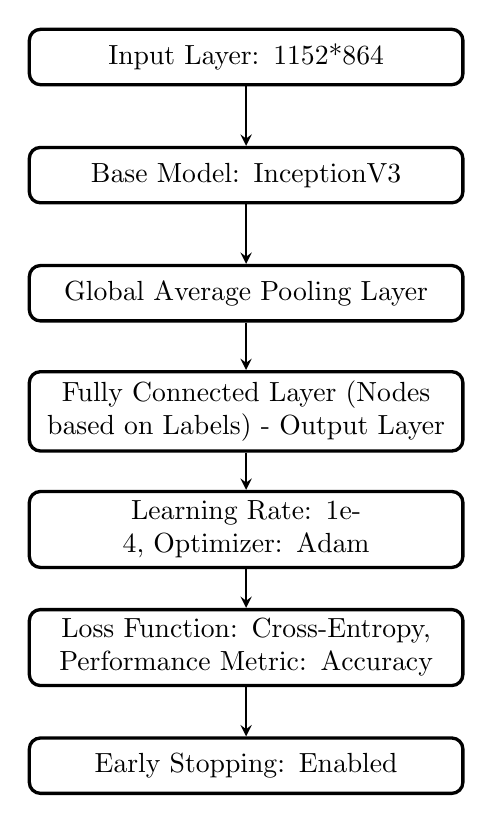
\begin{tikzpicture}[node distance=1.5cm,
        box/.style={
            rectangle,
            rounded corners,
            draw=black, very thick,
            text width=15em,
            minimum height=2em,
            text centered},
        arrow/.style={
            thick,
            ->,
            >=stealth}
        ]
    
        \node (collect) [box] {Input Layer: 1152*864};
        \node (mix) [box, below of=collect] {Base Model: InceptionV3};
        \node (train) [box, below of=mix] {Global Average Pooling Layer};
        \node (test) [box, below of=train] {Fully Connected Layer (Nodes based on Labels) - Output Layer};
        \node (evaluate) [box, below of=test] {Learning Rate: 1e-4, Optimizer: Adam};
        \node (rate) [box, below of=evaluate] {Loss Function: Cross-Entropy, Performance Metric: Accuracy};
        \node (improve) [box, below of=rate] {Early Stopping: Enabled};
        
        \draw [arrow] (collect) -- (mix);
        \draw [arrow] (mix) -- (train);
        \draw [arrow] (train) -- (test);
        \draw [arrow] (test) -- (evaluate);
        \draw [arrow] (evaluate) -- (rate);
        \draw [arrow] (rate) -- (improve);
        
        \end{tikzpicture}
\end{center}

\subsection{Future work}

\subsubsection{Enhancing Classification Methods}

\textbf{Broadening Classification Categories}

Current research shows promising outcomes using existing classification methods; however, these methods are confined to five categories. Expanding these categories could deepen insights into the correlation between cutting angles and sample quality, enhancing analytical precision. A broader classification spectrum could also improve predictions of optimal cutting angles for diverse tissue types and conditions.

\textbf{Transitioning to Linear Analytical Methods}

Introducing a more detailed classification could enable a shift from categorical to linear analytical methods. With sufficient categories acting as discrete points, linear relationships can be formed, allowing linear regression to accurately model the connection between cutting angles and sample quality.

Linear Discriminant Analysis (LDA) is valuable here, particularly for refining the determination of optimal cutting angles and correlating them with tissue quality. This approach simplifies predicting cutting parameters and enhances control over the tissue sectioning process.

\textbf{Challenges and Considerations}

Switching to a linear discriminant analysis framework poses significant challenges. Unlike binary classification models that provide probabilities, linear regression models explore direct relationships between variables, such as between cutting angles and tissue quality, which may not be straightforwardly linear.

Moreover, linear models require substantially more data, increasing both the duration and complexity of data collection and demanding greater computational resources. Current setups using TensorFlow and InceptionV3 models are already taxing GPU capacities, indicating a need for more advanced hardware and computational capabilities.

\textbf{Long-term Goals and Resource Needs}

These advancements are long-term objectives that require extensive resources and time. Research into linear discriminant analysis necessitates further theoretical study and practical experimentation. For instance, Jie Wen's "Robust Sparse Linear Discriminant Analysis" integrates sparsity into the LDA model, enhancing its robustness and suitability for complex applications.

% (如果可以增加相关论文证明观点:二分类和线性回归问题的对比和性能开销)


\subsubsection{Performance Enhancement and Optimization}

As this research progresses towards large-scale application, performance optimization emerges as a crucial challenge. This involves not only enhancing algorithm efficiency but also improving the scalability, stability, and deployment capabilities of the model framework, as well as optimizing the underlying programming languages and code.

To optimize the use of computational resources, adopting more efficient computing frameworks and parallel processing algorithms is essential. Utilizing distributed computing resources can significantly reduce model training times and enhance efficiency when processing large datasets. Moreover, considering constraints on energy consumption and computational costs, it's vital to optimize the model's computational architecture and parameter settings to maximize output within limited resources.

The article "Analysis of the Application Efficiency of TensorFlow and PyTorch in Convolutional Neural Network" highlights the differences between TensorFlow and PyTorch in processing convolutional neural networks\cite{6.2}. TensorFlow exhibits a lower error rate and smaller convergence steps, whereas PyTorch offers faster training speeds.

Pascal Fua's "Comparing Python, Go, and C++ on the N-Queens Problem" presents methods to optimize deep learning performance by comparing the efficiency of Python, Go, and C++ in solving the N-Queens problem.\cite{6.3} It was found that runtime languages have clear advantages in handling loops and data flows, suggesting that compiling tools like Numba, Cython, and Pybind11 can enhance performance in deep learning applications.




\subsubsection{Exploring the Impact of Additional Parameters on Cutting Quality}

In previous experiments, we established a model by setting the cutting angle as the independent variable and the cutting quality as the dependent variable. However, in reality, cutting quality may be influenced by other parameters such as cutting speed, feed rate (chip thickness), and tool wear.

In future work, if our focus is on the factors affecting cutting quality, research on these additional variables will be necessary. Indeed, the impact of these parameters on quality can be intuitively represented by a function:

\begin{equation}
Q = f(\theta, v, f, w)
\end{equation}

Here, $Q$ represents cutting quality, $\theta$ denotes the cutting angle, $v$ indicates the cutting speed, $f$ stands for the feed rate, and $w$ symbolizes tool wear. As for the specific form of this function, i.e., the weights of each parameter, it will require extensive experimental data for statistical analysis and fitting. This represents yet another challenge.

\subsubsection{Optimization of the Sectioning Process}

Our research also uncovered that real-time assessment of section quality during the cutting process, followed by adjustments based on those assessments, could significantly improve the quality of tissue sections.

The proposed feedback adjustment process involves installing a camera above the microtome to capture data from the samples being cut. This data is then analyzed in real-time by a pre-trained model, which assesses the quality of the sections. Based on this assessment, the cutting speed and angle parameters of the microtome can be adjusted to improve the quality of subsequent sections, thus ensuring controllable and consistent sample quality.

Implementing this system presents several challenges:

\begin{itemize}
    \item \textbf{Real-Time Image Processing:} A clear camera and an efficient real-time image processing system are needed to capture and process image data swiftly.
    \item \textbf{Powerful Computing Resources:} A pre-trained model and a powerful computer are required to quickly assess images and adjust the microtome's parameters based on the assessment.
    \item \textbf{Effective Control Interface:} An efficient control interface is necessary to ensure that the adjusted parameters are promptly communicated to the microtome.
    \item \textbf{Time Efficiency:} The entire system must operate within the brief intervals between cuts.
\end{itemize}

A pertinent example can be found in the study "Convolutional neural networks applied to microtomy: Identifying the trimming-end cutting routine on paraffin-embedded tissue blocks"\cite{6.4}. This research automated the sectioning process by monitoring it with a camera, analyzing the images with a CNN, and adjusting the microtome parameters based on the analysis. This integration of the microtome, camera, and deep learning model provides a feasible solution for real-time assessment and adjustment of cutting parameters during the sectioning process.


\subsection{Conclusions}

This research has significantly advanced our understanding of optimizing biopsy parameters through the application of deep learning techniques to biomedical tissue sectioning devices. By employing sophisticated convolutional neural networks, particularly through the adaptation of the InceptionV3 model via transfer learning, the study has demonstrated a robust framework capable of assessing the quality of tissue sections with high precision. This approach not only improves the accuracy of tissue sample analysis but also introduces a paradigm shift in the operational methodology of tissue sectioning.

By evaluating the quality of sections at different angles, we have discovered the relationship between the cutting angle and the quality of the sections. This provides us with a feasible method to improve the quality of sections in the future. In addition, the application of this model in different types of tissues (including fish ovaries and lung tissues) has confirmed its wide adaptability and potential for promotion, indicating that it is suitable for various tissue sections and research tasks.

However, the study also highlighted the limitations of traditional image preprocessing techniques. Initial attempts to enhance model performance through image preprocessing did not yield significant improvements and, in some cases, potentially obscured critical details necessary for accurate classification. This finding suggests that maintaining the integrity of original image data might be more beneficial than applying aggressive preprocessing techniques.

The research further explores enhancing the tissue slicing process through the expansion of classification methods and performance optimization. This includes integrating a greater number of classification categories and linear analysis methods such as Linear Discriminant Analysis (LDA), to more precisely understand the relationship between cutting parameters and sample quality. Concurrently, adopting more efficient computational frameworks and parallel processing techniques to optimize performance, as well as exploring additional parameters such as cutting speed and feed rate, will enhance the predictive capability of the model and the quality of tissue slices. Moreover, the implementation of a real-time feedback system, utilizing machine learning to dynamically adjust cutting parameters, will propel histological preparation towards automation, ensuring more consistent and high-quality tissue slices.

In conclusion, this project not only demonstrates the important role of deep learning in biomedical research and applications, but also provides feasibility for the further improvement of tissue sectioning technology. The combination of these technologies can bring improvements to biological sectioning equipment, provide a possible solution to improve the yield rate of tissue samples and the efficiency of sectioning. This research provides new ideas and methods for future tissue sectioning technology, and is expected to have a profound impact in the field of biomedicine.

% 总之,该项目不仅体现了深度学习在生物医学研究和应用中的重要作用,而且为组织切片技术的进一步提高提供了可行性。将这些技术的有机结合能够为生物切片设备带来改进,提高组织样本的良品率及提高切片效率提供了一个可能的解决方案。这一研究为未来的组织切片技术提供了新的思路和方法,有望在生物医学领域产生深远的影响。

\FloatBarrier % Now the table doesn't flow over to any other sections





\section{Project management, consideration of sustainability and health and safety}
\subsection{Subsection 5.1}
\subsection{Subsection 5.2}

\label{sec:conclusion}
%甘特图





%参考文献
\input{Misc/reference.tex}


%附录
% Appendix
%\appendix
%\pagenumbering{roman}
%\input{6.Appendix/appendix_A.tex}
%\input{6.Appendix/appendix_B.tex}
%\input{6.Appendix/appendix_C.tex}

%Example部分用于存放各种样例
\newpage
% \input{Example/example.tex}

\end{document} 